
% Default to the notebook output style

    


% Inherit from the specified cell style.




    
\documentclass[11pt]{article}

    
    
    \usepackage[T1]{fontenc}
    % Nicer default font (+ math font) than Computer Modern for most use cases
    \usepackage{mathpazo}

    % Basic figure setup, for now with no caption control since it's done
    % automatically by Pandoc (which extracts ![](path) syntax from Markdown).
    \usepackage{graphicx}
    % We will generate all images so they have a width \maxwidth. This means
    % that they will get their normal width if they fit onto the page, but
    % are scaled down if they would overflow the margins.
    \makeatletter
    \def\maxwidth{\ifdim\Gin@nat@width>\linewidth\linewidth
    \else\Gin@nat@width\fi}
    \makeatother
    \let\Oldincludegraphics\includegraphics
    % Set max figure width to be 80% of text width, for now hardcoded.
    \renewcommand{\includegraphics}[1]{\Oldincludegraphics[width=.8\maxwidth]{#1}}
    % Ensure that by default, figures have no caption (until we provide a
    % proper Figure object with a Caption API and a way to capture that
    % in the conversion process - todo).
    \usepackage{caption}
    \DeclareCaptionLabelFormat{nolabel}{}
    \captionsetup{labelformat=nolabel}

    \usepackage{adjustbox} % Used to constrain images to a maximum size 
    \usepackage{xcolor} % Allow colors to be defined
    \usepackage{enumerate} % Needed for markdown enumerations to work
    \usepackage{geometry} % Used to adjust the document margins
    \usepackage{amsmath} % Equations
    \usepackage{amssymb} % Equations
    \usepackage{textcomp} % defines textquotesingle
    % Hack from http://tex.stackexchange.com/a/47451/13684:
    \AtBeginDocument{%
        \def\PYZsq{\textquotesingle}% Upright quotes in Pygmentized code
    }
    \usepackage{upquote} % Upright quotes for verbatim code
    \usepackage{eurosym} % defines \euro
    \usepackage[mathletters]{ucs} % Extended unicode (utf-8) support
    \usepackage[utf8x]{inputenc} % Allow utf-8 characters in the tex document
    \usepackage{fancyvrb} % verbatim replacement that allows latex
    \usepackage{grffile} % extends the file name processing of package graphics 
                         % to support a larger range 
    % The hyperref package gives us a pdf with properly built
    % internal navigation ('pdf bookmarks' for the table of contents,
    % internal cross-reference links, web links for URLs, etc.)
    \usepackage{hyperref}
    \usepackage{longtable} % longtable support required by pandoc >1.10
    \usepackage{booktabs}  % table support for pandoc > 1.12.2
    \usepackage[inline]{enumitem} % IRkernel/repr support (it uses the enumerate* environment)
    \usepackage[normalem]{ulem} % ulem is needed to support strikethroughs (\sout)
                                % normalem makes italics be italics, not underlines
    

    
    
    % Colors for the hyperref package
    \definecolor{urlcolor}{rgb}{0,.145,.698}
    \definecolor{linkcolor}{rgb}{.71,0.21,0.01}
    \definecolor{citecolor}{rgb}{.12,.54,.11}

    % ANSI colors
    \definecolor{ansi-black}{HTML}{3E424D}
    \definecolor{ansi-black-intense}{HTML}{282C36}
    \definecolor{ansi-red}{HTML}{E75C58}
    \definecolor{ansi-red-intense}{HTML}{B22B31}
    \definecolor{ansi-green}{HTML}{00A250}
    \definecolor{ansi-green-intense}{HTML}{007427}
    \definecolor{ansi-yellow}{HTML}{DDB62B}
    \definecolor{ansi-yellow-intense}{HTML}{B27D12}
    \definecolor{ansi-blue}{HTML}{208FFB}
    \definecolor{ansi-blue-intense}{HTML}{0065CA}
    \definecolor{ansi-magenta}{HTML}{D160C4}
    \definecolor{ansi-magenta-intense}{HTML}{A03196}
    \definecolor{ansi-cyan}{HTML}{60C6C8}
    \definecolor{ansi-cyan-intense}{HTML}{258F8F}
    \definecolor{ansi-white}{HTML}{C5C1B4}
    \definecolor{ansi-white-intense}{HTML}{A1A6B2}

    % commands and environments needed by pandoc snippets
    % extracted from the output of `pandoc -s`
    \providecommand{\tightlist}{%
      \setlength{\itemsep}{0pt}\setlength{\parskip}{0pt}}
    \DefineVerbatimEnvironment{Highlighting}{Verbatim}{commandchars=\\\{\}}
    % Add ',fontsize=\small' for more characters per line
    \newenvironment{Shaded}{}{}
    \newcommand{\KeywordTok}[1]{\textcolor[rgb]{0.00,0.44,0.13}{\textbf{{#1}}}}
    \newcommand{\DataTypeTok}[1]{\textcolor[rgb]{0.56,0.13,0.00}{{#1}}}
    \newcommand{\DecValTok}[1]{\textcolor[rgb]{0.25,0.63,0.44}{{#1}}}
    \newcommand{\BaseNTok}[1]{\textcolor[rgb]{0.25,0.63,0.44}{{#1}}}
    \newcommand{\FloatTok}[1]{\textcolor[rgb]{0.25,0.63,0.44}{{#1}}}
    \newcommand{\CharTok}[1]{\textcolor[rgb]{0.25,0.44,0.63}{{#1}}}
    \newcommand{\StringTok}[1]{\textcolor[rgb]{0.25,0.44,0.63}{{#1}}}
    \newcommand{\CommentTok}[1]{\textcolor[rgb]{0.38,0.63,0.69}{\textit{{#1}}}}
    \newcommand{\OtherTok}[1]{\textcolor[rgb]{0.00,0.44,0.13}{{#1}}}
    \newcommand{\AlertTok}[1]{\textcolor[rgb]{1.00,0.00,0.00}{\textbf{{#1}}}}
    \newcommand{\FunctionTok}[1]{\textcolor[rgb]{0.02,0.16,0.49}{{#1}}}
    \newcommand{\RegionMarkerTok}[1]{{#1}}
    \newcommand{\ErrorTok}[1]{\textcolor[rgb]{1.00,0.00,0.00}{\textbf{{#1}}}}
    \newcommand{\NormalTok}[1]{{#1}}
    
    % Additional commands for more recent versions of Pandoc
    \newcommand{\ConstantTok}[1]{\textcolor[rgb]{0.53,0.00,0.00}{{#1}}}
    \newcommand{\SpecialCharTok}[1]{\textcolor[rgb]{0.25,0.44,0.63}{{#1}}}
    \newcommand{\VerbatimStringTok}[1]{\textcolor[rgb]{0.25,0.44,0.63}{{#1}}}
    \newcommand{\SpecialStringTok}[1]{\textcolor[rgb]{0.73,0.40,0.53}{{#1}}}
    \newcommand{\ImportTok}[1]{{#1}}
    \newcommand{\DocumentationTok}[1]{\textcolor[rgb]{0.73,0.13,0.13}{\textit{{#1}}}}
    \newcommand{\AnnotationTok}[1]{\textcolor[rgb]{0.38,0.63,0.69}{\textbf{\textit{{#1}}}}}
    \newcommand{\CommentVarTok}[1]{\textcolor[rgb]{0.38,0.63,0.69}{\textbf{\textit{{#1}}}}}
    \newcommand{\VariableTok}[1]{\textcolor[rgb]{0.10,0.09,0.49}{{#1}}}
    \newcommand{\ControlFlowTok}[1]{\textcolor[rgb]{0.00,0.44,0.13}{\textbf{{#1}}}}
    \newcommand{\OperatorTok}[1]{\textcolor[rgb]{0.40,0.40,0.40}{{#1}}}
    \newcommand{\BuiltInTok}[1]{{#1}}
    \newcommand{\ExtensionTok}[1]{{#1}}
    \newcommand{\PreprocessorTok}[1]{\textcolor[rgb]{0.74,0.48,0.00}{{#1}}}
    \newcommand{\AttributeTok}[1]{\textcolor[rgb]{0.49,0.56,0.16}{{#1}}}
    \newcommand{\InformationTok}[1]{\textcolor[rgb]{0.38,0.63,0.69}{\textbf{\textit{{#1}}}}}
    \newcommand{\WarningTok}[1]{\textcolor[rgb]{0.38,0.63,0.69}{\textbf{\textit{{#1}}}}}
    
    
    % Define a nice break command that doesn't care if a line doesn't already
    % exist.
    \def\br{\hspace*{\fill} \\* }
    % Math Jax compatability definitions
    \def\gt{>}
    \def\lt{<}
    % Document parameters
    \title{HMM Tagger}
    
    
    

    % Pygments definitions
    
\makeatletter
\def\PY@reset{\let\PY@it=\relax \let\PY@bf=\relax%
    \let\PY@ul=\relax \let\PY@tc=\relax%
    \let\PY@bc=\relax \let\PY@ff=\relax}
\def\PY@tok#1{\csname PY@tok@#1\endcsname}
\def\PY@toks#1+{\ifx\relax#1\empty\else%
    \PY@tok{#1}\expandafter\PY@toks\fi}
\def\PY@do#1{\PY@bc{\PY@tc{\PY@ul{%
    \PY@it{\PY@bf{\PY@ff{#1}}}}}}}
\def\PY#1#2{\PY@reset\PY@toks#1+\relax+\PY@do{#2}}

\expandafter\def\csname PY@tok@vc\endcsname{\def\PY@tc##1{\textcolor[rgb]{0.10,0.09,0.49}{##1}}}
\expandafter\def\csname PY@tok@sh\endcsname{\def\PY@tc##1{\textcolor[rgb]{0.73,0.13,0.13}{##1}}}
\expandafter\def\csname PY@tok@kr\endcsname{\let\PY@bf=\textbf\def\PY@tc##1{\textcolor[rgb]{0.00,0.50,0.00}{##1}}}
\expandafter\def\csname PY@tok@k\endcsname{\let\PY@bf=\textbf\def\PY@tc##1{\textcolor[rgb]{0.00,0.50,0.00}{##1}}}
\expandafter\def\csname PY@tok@c\endcsname{\let\PY@it=\textit\def\PY@tc##1{\textcolor[rgb]{0.25,0.50,0.50}{##1}}}
\expandafter\def\csname PY@tok@il\endcsname{\def\PY@tc##1{\textcolor[rgb]{0.40,0.40,0.40}{##1}}}
\expandafter\def\csname PY@tok@cpf\endcsname{\let\PY@it=\textit\def\PY@tc##1{\textcolor[rgb]{0.25,0.50,0.50}{##1}}}
\expandafter\def\csname PY@tok@gt\endcsname{\def\PY@tc##1{\textcolor[rgb]{0.00,0.27,0.87}{##1}}}
\expandafter\def\csname PY@tok@gp\endcsname{\let\PY@bf=\textbf\def\PY@tc##1{\textcolor[rgb]{0.00,0.00,0.50}{##1}}}
\expandafter\def\csname PY@tok@nn\endcsname{\let\PY@bf=\textbf\def\PY@tc##1{\textcolor[rgb]{0.00,0.00,1.00}{##1}}}
\expandafter\def\csname PY@tok@kc\endcsname{\let\PY@bf=\textbf\def\PY@tc##1{\textcolor[rgb]{0.00,0.50,0.00}{##1}}}
\expandafter\def\csname PY@tok@ni\endcsname{\let\PY@bf=\textbf\def\PY@tc##1{\textcolor[rgb]{0.60,0.60,0.60}{##1}}}
\expandafter\def\csname PY@tok@cp\endcsname{\def\PY@tc##1{\textcolor[rgb]{0.74,0.48,0.00}{##1}}}
\expandafter\def\csname PY@tok@nd\endcsname{\def\PY@tc##1{\textcolor[rgb]{0.67,0.13,1.00}{##1}}}
\expandafter\def\csname PY@tok@gh\endcsname{\let\PY@bf=\textbf\def\PY@tc##1{\textcolor[rgb]{0.00,0.00,0.50}{##1}}}
\expandafter\def\csname PY@tok@vi\endcsname{\def\PY@tc##1{\textcolor[rgb]{0.10,0.09,0.49}{##1}}}
\expandafter\def\csname PY@tok@nf\endcsname{\def\PY@tc##1{\textcolor[rgb]{0.00,0.00,1.00}{##1}}}
\expandafter\def\csname PY@tok@mf\endcsname{\def\PY@tc##1{\textcolor[rgb]{0.40,0.40,0.40}{##1}}}
\expandafter\def\csname PY@tok@sa\endcsname{\def\PY@tc##1{\textcolor[rgb]{0.73,0.13,0.13}{##1}}}
\expandafter\def\csname PY@tok@s1\endcsname{\def\PY@tc##1{\textcolor[rgb]{0.73,0.13,0.13}{##1}}}
\expandafter\def\csname PY@tok@se\endcsname{\let\PY@bf=\textbf\def\PY@tc##1{\textcolor[rgb]{0.73,0.40,0.13}{##1}}}
\expandafter\def\csname PY@tok@gu\endcsname{\let\PY@bf=\textbf\def\PY@tc##1{\textcolor[rgb]{0.50,0.00,0.50}{##1}}}
\expandafter\def\csname PY@tok@s2\endcsname{\def\PY@tc##1{\textcolor[rgb]{0.73,0.13,0.13}{##1}}}
\expandafter\def\csname PY@tok@na\endcsname{\def\PY@tc##1{\textcolor[rgb]{0.49,0.56,0.16}{##1}}}
\expandafter\def\csname PY@tok@nv\endcsname{\def\PY@tc##1{\textcolor[rgb]{0.10,0.09,0.49}{##1}}}
\expandafter\def\csname PY@tok@go\endcsname{\def\PY@tc##1{\textcolor[rgb]{0.53,0.53,0.53}{##1}}}
\expandafter\def\csname PY@tok@fm\endcsname{\def\PY@tc##1{\textcolor[rgb]{0.00,0.00,1.00}{##1}}}
\expandafter\def\csname PY@tok@c1\endcsname{\let\PY@it=\textit\def\PY@tc##1{\textcolor[rgb]{0.25,0.50,0.50}{##1}}}
\expandafter\def\csname PY@tok@mi\endcsname{\def\PY@tc##1{\textcolor[rgb]{0.40,0.40,0.40}{##1}}}
\expandafter\def\csname PY@tok@sr\endcsname{\def\PY@tc##1{\textcolor[rgb]{0.73,0.40,0.53}{##1}}}
\expandafter\def\csname PY@tok@cm\endcsname{\let\PY@it=\textit\def\PY@tc##1{\textcolor[rgb]{0.25,0.50,0.50}{##1}}}
\expandafter\def\csname PY@tok@kp\endcsname{\def\PY@tc##1{\textcolor[rgb]{0.00,0.50,0.00}{##1}}}
\expandafter\def\csname PY@tok@sb\endcsname{\def\PY@tc##1{\textcolor[rgb]{0.73,0.13,0.13}{##1}}}
\expandafter\def\csname PY@tok@nb\endcsname{\def\PY@tc##1{\textcolor[rgb]{0.00,0.50,0.00}{##1}}}
\expandafter\def\csname PY@tok@gr\endcsname{\def\PY@tc##1{\textcolor[rgb]{1.00,0.00,0.00}{##1}}}
\expandafter\def\csname PY@tok@kd\endcsname{\let\PY@bf=\textbf\def\PY@tc##1{\textcolor[rgb]{0.00,0.50,0.00}{##1}}}
\expandafter\def\csname PY@tok@vm\endcsname{\def\PY@tc##1{\textcolor[rgb]{0.10,0.09,0.49}{##1}}}
\expandafter\def\csname PY@tok@mh\endcsname{\def\PY@tc##1{\textcolor[rgb]{0.40,0.40,0.40}{##1}}}
\expandafter\def\csname PY@tok@ge\endcsname{\let\PY@it=\textit}
\expandafter\def\csname PY@tok@kt\endcsname{\def\PY@tc##1{\textcolor[rgb]{0.69,0.00,0.25}{##1}}}
\expandafter\def\csname PY@tok@si\endcsname{\let\PY@bf=\textbf\def\PY@tc##1{\textcolor[rgb]{0.73,0.40,0.53}{##1}}}
\expandafter\def\csname PY@tok@gs\endcsname{\let\PY@bf=\textbf}
\expandafter\def\csname PY@tok@kn\endcsname{\let\PY@bf=\textbf\def\PY@tc##1{\textcolor[rgb]{0.00,0.50,0.00}{##1}}}
\expandafter\def\csname PY@tok@no\endcsname{\def\PY@tc##1{\textcolor[rgb]{0.53,0.00,0.00}{##1}}}
\expandafter\def\csname PY@tok@nl\endcsname{\def\PY@tc##1{\textcolor[rgb]{0.63,0.63,0.00}{##1}}}
\expandafter\def\csname PY@tok@err\endcsname{\def\PY@bc##1{\setlength{\fboxsep}{0pt}\fcolorbox[rgb]{1.00,0.00,0.00}{1,1,1}{\strut ##1}}}
\expandafter\def\csname PY@tok@ow\endcsname{\let\PY@bf=\textbf\def\PY@tc##1{\textcolor[rgb]{0.67,0.13,1.00}{##1}}}
\expandafter\def\csname PY@tok@ss\endcsname{\def\PY@tc##1{\textcolor[rgb]{0.10,0.09,0.49}{##1}}}
\expandafter\def\csname PY@tok@gi\endcsname{\def\PY@tc##1{\textcolor[rgb]{0.00,0.63,0.00}{##1}}}
\expandafter\def\csname PY@tok@mb\endcsname{\def\PY@tc##1{\textcolor[rgb]{0.40,0.40,0.40}{##1}}}
\expandafter\def\csname PY@tok@bp\endcsname{\def\PY@tc##1{\textcolor[rgb]{0.00,0.50,0.00}{##1}}}
\expandafter\def\csname PY@tok@dl\endcsname{\def\PY@tc##1{\textcolor[rgb]{0.73,0.13,0.13}{##1}}}
\expandafter\def\csname PY@tok@mo\endcsname{\def\PY@tc##1{\textcolor[rgb]{0.40,0.40,0.40}{##1}}}
\expandafter\def\csname PY@tok@s\endcsname{\def\PY@tc##1{\textcolor[rgb]{0.73,0.13,0.13}{##1}}}
\expandafter\def\csname PY@tok@m\endcsname{\def\PY@tc##1{\textcolor[rgb]{0.40,0.40,0.40}{##1}}}
\expandafter\def\csname PY@tok@ne\endcsname{\let\PY@bf=\textbf\def\PY@tc##1{\textcolor[rgb]{0.82,0.25,0.23}{##1}}}
\expandafter\def\csname PY@tok@vg\endcsname{\def\PY@tc##1{\textcolor[rgb]{0.10,0.09,0.49}{##1}}}
\expandafter\def\csname PY@tok@sd\endcsname{\let\PY@it=\textit\def\PY@tc##1{\textcolor[rgb]{0.73,0.13,0.13}{##1}}}
\expandafter\def\csname PY@tok@cs\endcsname{\let\PY@it=\textit\def\PY@tc##1{\textcolor[rgb]{0.25,0.50,0.50}{##1}}}
\expandafter\def\csname PY@tok@ch\endcsname{\let\PY@it=\textit\def\PY@tc##1{\textcolor[rgb]{0.25,0.50,0.50}{##1}}}
\expandafter\def\csname PY@tok@w\endcsname{\def\PY@tc##1{\textcolor[rgb]{0.73,0.73,0.73}{##1}}}
\expandafter\def\csname PY@tok@gd\endcsname{\def\PY@tc##1{\textcolor[rgb]{0.63,0.00,0.00}{##1}}}
\expandafter\def\csname PY@tok@nt\endcsname{\let\PY@bf=\textbf\def\PY@tc##1{\textcolor[rgb]{0.00,0.50,0.00}{##1}}}
\expandafter\def\csname PY@tok@sx\endcsname{\def\PY@tc##1{\textcolor[rgb]{0.00,0.50,0.00}{##1}}}
\expandafter\def\csname PY@tok@o\endcsname{\def\PY@tc##1{\textcolor[rgb]{0.40,0.40,0.40}{##1}}}
\expandafter\def\csname PY@tok@nc\endcsname{\let\PY@bf=\textbf\def\PY@tc##1{\textcolor[rgb]{0.00,0.00,1.00}{##1}}}
\expandafter\def\csname PY@tok@sc\endcsname{\def\PY@tc##1{\textcolor[rgb]{0.73,0.13,0.13}{##1}}}

\def\PYZbs{\char`\\}
\def\PYZus{\char`\_}
\def\PYZob{\char`\{}
\def\PYZcb{\char`\}}
\def\PYZca{\char`\^}
\def\PYZam{\char`\&}
\def\PYZlt{\char`\<}
\def\PYZgt{\char`\>}
\def\PYZsh{\char`\#}
\def\PYZpc{\char`\%}
\def\PYZdl{\char`\$}
\def\PYZhy{\char`\-}
\def\PYZsq{\char`\'}
\def\PYZdq{\char`\"}
\def\PYZti{\char`\~}
% for compatibility with earlier versions
\def\PYZat{@}
\def\PYZlb{[}
\def\PYZrb{]}
\makeatother


    % Exact colors from NB
    \definecolor{incolor}{rgb}{0.0, 0.0, 0.5}
    \definecolor{outcolor}{rgb}{0.545, 0.0, 0.0}



    
    % Prevent overflowing lines due to hard-to-break entities
    \sloppy 
    % Setup hyperref package
    \hypersetup{
      breaklinks=true,  % so long urls are correctly broken across lines
      colorlinks=true,
      urlcolor=urlcolor,
      linkcolor=linkcolor,
      citecolor=citecolor,
      }
    % Slightly bigger margins than the latex defaults
    
    \geometry{verbose,tmargin=1in,bmargin=1in,lmargin=1in,rmargin=1in}
    
    

    \begin{document}
    
    
    \maketitle
    
    

    
    \hypertarget{project-part-of-speech-tagging-with-hidden-markov-models}{%
\subsection{\# Project: Part of Speech Tagging with Hidden Markov
Models}\label{project-part-of-speech-tagging-with-hidden-markov-models}}

\hypertarget{introduction}{%
\subsubsection{Introduction}\label{introduction}}

Part of speech tagging is the process of determining the syntactic
category of a word from the words in its surrounding context. It is
often used to help disambiguate natural language phrases because it can
be done quickly with high accuracy. Tagging can be used for many NLP
tasks like determining correct pronunciation during speech synthesis
(for example, \emph{dis}-count as a noun vs dis-\emph{count} as a verb),
for information retrieval, and for word sense disambiguation.

In this notebook, you'll use the
\href{http://pomegranate.readthedocs.io/}{Pomegranate} library to build
a hidden Markov model for part of speech tagging using a ``universal''
tagset. Hidden Markov models have been able to achieve
\href{http://www.coli.uni-saarland.de/~thorsten/publications/Brants-ANLP00.pdf}{\textgreater{}96\%
tag accuracy with larger tagsets on realistic text corpora}. Hidden
Markov models have also been used for speech recognition and speech
generation, machine translation, gene recognition for bioinformatics,
and human gesture recognition for computer vision, and more.

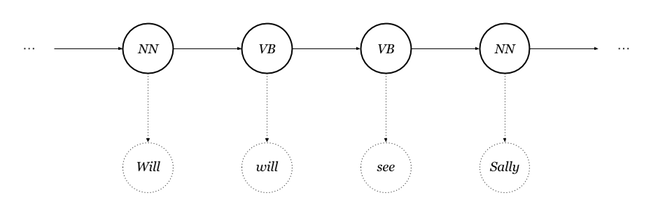
\includegraphics{_post-hmm.png}

The notebook already contains some code to get you started. You only
need to add some new functionality in the areas indicated to complete
the project; you will not need to modify the included code beyond what
is requested. Sections that begin with \textbf{`IMPLEMENTATION'} in the
header indicate that you must provide code in the block that follows.
Instructions will be provided for each section, and the specifics of the
implementation are marked in the code block with a `TODO' statement.
Please be sure to read the instructions carefully!

    \textbf{Note:} Once you have completed all of the code implementations,
you need to finalize your work by exporting the iPython Notebook as an
HTML document. Before exporting the notebook to html, all of the code
cells need to have been run so that reviewers can see the final
implementation and output. You must then \textbf{export the notebook} by
running the last cell in the notebook, or by using the menu above and
navigating to \textbf{File -\textgreater{} Download as -\textgreater{}
HTML (.html)} Your submissions should include both the \texttt{html} and
\texttt{ipynb} files.

    \textbf{Note:} Code and Markdown cells can be executed using the
\texttt{Shift\ +\ Enter} keyboard shortcut. Markdown cells can be edited
by double-clicking the cell to enter edit mode.

    \hypertarget{the-road-ahead}{%
\subsubsection{The Road Ahead}\label{the-road-ahead}}

You must complete Steps 1-3 below to pass the project. The section on
Step 4 includes references \& resources you can use to further explore
HMM taggers.

\begin{itemize}
\tightlist
\item
  Section \ref{step-1-read-and-preprocess-the-dataset}: Review the
  provided interface to load and access the text corpus
\item
  Section \ref{step-2-build-a-most-frequent-class-tagger}: Build a Most
  Frequent Class tagger to use as a baseline
\item
  Section \ref{step-3-build-an-hmm-tagger}: Build an HMM Part of Speech
  tagger and compare to the MFC baseline
\item
  Section \ref{step-4-5boptional5d-improving-model-performance}:
  (Optional) Improve the HMM tagger
\end{itemize}

    \begin{Verbatim}[commandchars=\\\{\}]
{\color{incolor}In [{\color{incolor}179}]:} \PY{c+c1}{\PYZsh{} Jupyter \PYZdq{}magic methods\PYZdq{} \PYZhy{}\PYZhy{} only need to be run once per kernel restart}
          \PY{o}{\PYZpc{}}\PY{k}{load\PYZus{}ext} autoreload
          \PY{o}{\PYZpc{}}\PY{k}{aimport} helpers, tests
          \PY{o}{\PYZpc{}}\PY{k}{autoreload} 1
\end{Verbatim}


    \begin{Verbatim}[commandchars=\\\{\}]
The autoreload extension is already loaded. To reload it, use:
  \%reload\_ext autoreload

    \end{Verbatim}

    \begin{Verbatim}[commandchars=\\\{\}]
{\color{incolor}In [{\color{incolor}180}]:} \PY{c+c1}{\PYZsh{} import python modules \PYZhy{}\PYZhy{} this cell needs to be run again if you make changes to any of the files}
          \PY{k+kn}{import} \PY{n+nn}{matplotlib}\PY{n+nn}{.}\PY{n+nn}{pyplot} \PY{k}{as} \PY{n+nn}{plt}
          \PY{k+kn}{import} \PY{n+nn}{numpy} \PY{k}{as} \PY{n+nn}{np}
          
          \PY{k+kn}{from} \PY{n+nn}{IPython}\PY{n+nn}{.}\PY{n+nn}{core}\PY{n+nn}{.}\PY{n+nn}{display} \PY{k}{import} \PY{n}{HTML}
          \PY{k+kn}{from} \PY{n+nn}{itertools} \PY{k}{import} \PY{n}{chain}
          \PY{k+kn}{from} \PY{n+nn}{collections} \PY{k}{import} \PY{n}{Counter}\PY{p}{,} \PY{n}{defaultdict}
          \PY{k+kn}{from} \PY{n+nn}{helpers} \PY{k}{import} \PY{n}{show\PYZus{}model}\PY{p}{,} \PY{n}{Dataset}
          \PY{k+kn}{from} \PY{n+nn}{pomegranate} \PY{k}{import} \PY{n}{State}\PY{p}{,} \PY{n}{HiddenMarkovModel}\PY{p}{,} \PY{n}{DiscreteDistribution}
\end{Verbatim}


    \hypertarget{step-1-read-and-preprocess-the-dataset}{%
\subsection{\#\# Step 1: Read and preprocess the
dataset}\label{step-1-read-and-preprocess-the-dataset}}

We'll start by reading in a text corpus and splitting it into a training
and testing dataset. The data set is a copy of the
\href{https://en.wikipedia.org/wiki/Brown_Corpus}{Brown corpus}
(originally from the \href{https://www.nltk.org/}{NLTK} library) that
has already been pre-processed to only include the
\href{https://arxiv.org/pdf/1104.2086.pdf}{universal tagset}. You should
expect to get slightly higher accuracy using this simplified tagset than
the same model would achieve on a larger tagset like the full
\href{https://www.ling.upenn.edu/courses/Fall_2003/ling001/penn_treebank_pos.html}{Penn
treebank tagset}, but the process you'll follow would be the same.

The \texttt{Dataset} class provided in helpers.py will read and parse
the corpus. You can generate your own datasets compatible with the
reader by writing them to the following format. The dataset is stored in
plaintext as a collection of words and corresponding tags. Each sentence
starts with a unique identifier on the first line, followed by one
tab-separated word/tag pair on each following line. Sentences are
separated by a single blank line.

Example from the Brown corpus.

\begin{verbatim}
b100-38532
Perhaps ADV
it  PRON
was VERB
right   ADJ
;   .
;   .

b100-35577
...
\end{verbatim}

    \begin{Verbatim}[commandchars=\\\{\}]
{\color{incolor}In [{\color{incolor}181}]:} \PY{n}{data} \PY{o}{=} \PY{n}{Dataset}\PY{p}{(}\PY{l+s+s2}{\PYZdq{}}\PY{l+s+s2}{tags\PYZhy{}universal.txt}\PY{l+s+s2}{\PYZdq{}}\PY{p}{,} \PY{l+s+s2}{\PYZdq{}}\PY{l+s+s2}{brown\PYZhy{}universal.txt}\PY{l+s+s2}{\PYZdq{}}\PY{p}{,} \PY{n}{train\PYZus{}test\PYZus{}split}\PY{o}{=}\PY{l+m+mf}{0.8}\PY{p}{)}
          
          \PY{n+nb}{print}\PY{p}{(}\PY{l+s+s2}{\PYZdq{}}\PY{l+s+s2}{There are }\PY{l+s+si}{\PYZob{}\PYZcb{}}\PY{l+s+s2}{ sentences in the corpus.}\PY{l+s+s2}{\PYZdq{}}\PY{o}{.}\PY{n}{format}\PY{p}{(}\PY{n+nb}{len}\PY{p}{(}\PY{n}{data}\PY{p}{)}\PY{p}{)}\PY{p}{)}
          \PY{n+nb}{print}\PY{p}{(}\PY{l+s+s2}{\PYZdq{}}\PY{l+s+s2}{There are }\PY{l+s+si}{\PYZob{}\PYZcb{}}\PY{l+s+s2}{ sentences in the training set.}\PY{l+s+s2}{\PYZdq{}}\PY{o}{.}\PY{n}{format}\PY{p}{(}\PY{n+nb}{len}\PY{p}{(}\PY{n}{data}\PY{o}{.}\PY{n}{training\PYZus{}set}\PY{p}{)}\PY{p}{)}\PY{p}{)}
          \PY{n+nb}{print}\PY{p}{(}\PY{l+s+s2}{\PYZdq{}}\PY{l+s+s2}{There are }\PY{l+s+si}{\PYZob{}\PYZcb{}}\PY{l+s+s2}{ sentences in the testing set.}\PY{l+s+s2}{\PYZdq{}}\PY{o}{.}\PY{n}{format}\PY{p}{(}\PY{n+nb}{len}\PY{p}{(}\PY{n}{data}\PY{o}{.}\PY{n}{testing\PYZus{}set}\PY{p}{)}\PY{p}{)}\PY{p}{)}
          
          \PY{k}{assert} \PY{n+nb}{len}\PY{p}{(}\PY{n}{data}\PY{p}{)} \PY{o}{==} \PY{n+nb}{len}\PY{p}{(}\PY{n}{data}\PY{o}{.}\PY{n}{training\PYZus{}set}\PY{p}{)} \PY{o}{+} \PY{n+nb}{len}\PY{p}{(}\PY{n}{data}\PY{o}{.}\PY{n}{testing\PYZus{}set}\PY{p}{)}\PY{p}{,} \PYZbs{}
                 \PY{l+s+s2}{\PYZdq{}}\PY{l+s+s2}{The number of sentences in the training set + testing set should sum to the number of sentences in the corpus}\PY{l+s+s2}{\PYZdq{}}
\end{Verbatim}


    \begin{Verbatim}[commandchars=\\\{\}]
There are 57340 sentences in the corpus.
There are 45872 sentences in the training set.
There are 11468 sentences in the testing set.

    \end{Verbatim}

    \hypertarget{the-dataset-interface}{%
\subsubsection{The Dataset Interface}\label{the-dataset-interface}}

You can access (mostly) immutable references to the dataset through a
simple interface provided through the \texttt{Dataset} class, which
represents an iterable collection of sentences along with easy access to
partitions of the data for training \& testing. Review the reference
below, then run and review the next few cells to make sure you
understand the interface before moving on to the next step.

\begin{verbatim}
Dataset-only Attributes:
    training_set - reference to a Subset object containing the samples for training
    testing_set - reference to a Subset object containing the samples for testing

Dataset & Subset Attributes:
    sentences - a dictionary with an entry {sentence_key: Sentence()} for each sentence in the corpus
    keys - an immutable ordered (not sorted) collection of the sentence_keys for the corpus
    vocab - an immutable collection of the unique words in the corpus
    tagset - an immutable collection of the unique tags in the corpus
    X - returns an array of words grouped by sentences ((w11, w12, w13, ...), (w21, w22, w23, ...), ...)
    Y - returns an array of tags grouped by sentences ((t11, t12, t13, ...), (t21, t22, t23, ...), ...)
    N - returns the number of distinct samples (individual words or tags) in the dataset

Methods:
    stream() - returns an flat iterable over all (word, tag) pairs across all sentences in the corpus
    __iter__() - returns an iterable over the data as (sentence_key, Sentence()) pairs
    __len__() - returns the nubmer of sentences in the dataset
\end{verbatim}

For example, consider a Subset, \texttt{subset}, of the sentences
\texttt{\{"s0":\ Sentence(("See",\ "Spot",\ "run"),\ ("VERB",\ "NOUN",\ "VERB")),\ "s1":\ Sentence(("Spot",\ "ran"),\ ("NOUN",\ "VERB"))\}}.
The subset will have these attributes:

\begin{verbatim}
subset.keys == {"s1", "s0"}  # unordered
subset.vocab == {"See", "run", "ran", "Spot"}  # unordered
subset.tagset == {"VERB", "NOUN"}  # unordered
subset.X == (("Spot", "ran"), ("See", "Spot", "run"))  # order matches .keys
subset.Y == (("NOUN", "VERB"), ("VERB", "NOUN", "VERB"))  # order matches .keys
subset.N == 7  # there are a total of seven observations over all sentences
len(subset) == 2  # because there are two sentences
\end{verbatim}

\textbf{Note:} The \texttt{Dataset} class is \emph{convenient}, but it
is \textbf{not} efficient. It is not suitable for huge datasets because
it stores multiple redundant copies of the same data.

    \hypertarget{sentences}{%
\paragraph{Sentences}\label{sentences}}

\texttt{Dataset.sentences} is a dictionary of all sentences in the
training corpus, each keyed to a unique sentence identifier. Each
\texttt{Sentence} is itself an object with two attributes: a tuple of
the words in the sentence named \texttt{words} and a tuple of the tag
corresponding to each word named \texttt{tags}.

    \begin{Verbatim}[commandchars=\\\{\}]
{\color{incolor}In [{\color{incolor}182}]:} \PY{n}{key} \PY{o}{=} \PY{l+s+s1}{\PYZsq{}}\PY{l+s+s1}{b100\PYZhy{}38532}\PY{l+s+s1}{\PYZsq{}}
          \PY{n+nb}{print}\PY{p}{(}\PY{l+s+s2}{\PYZdq{}}\PY{l+s+s2}{Sentence: }\PY{l+s+si}{\PYZob{}\PYZcb{}}\PY{l+s+s2}{\PYZdq{}}\PY{o}{.}\PY{n}{format}\PY{p}{(}\PY{n}{key}\PY{p}{)}\PY{p}{)}
          \PY{n+nb}{print}\PY{p}{(}\PY{l+s+s2}{\PYZdq{}}\PY{l+s+s2}{words:}\PY{l+s+se}{\PYZbs{}n}\PY{l+s+se}{\PYZbs{}t}\PY{l+s+si}{\PYZob{}!s\PYZcb{}}\PY{l+s+s2}{\PYZdq{}}\PY{o}{.}\PY{n}{format}\PY{p}{(}\PY{n}{data}\PY{o}{.}\PY{n}{sentences}\PY{p}{[}\PY{n}{key}\PY{p}{]}\PY{o}{.}\PY{n}{words}\PY{p}{)}\PY{p}{)}
          \PY{n+nb}{print}\PY{p}{(}\PY{l+s+s2}{\PYZdq{}}\PY{l+s+s2}{tags:}\PY{l+s+se}{\PYZbs{}n}\PY{l+s+se}{\PYZbs{}t}\PY{l+s+si}{\PYZob{}!s\PYZcb{}}\PY{l+s+s2}{\PYZdq{}}\PY{o}{.}\PY{n}{format}\PY{p}{(}\PY{n}{data}\PY{o}{.}\PY{n}{sentences}\PY{p}{[}\PY{n}{key}\PY{p}{]}\PY{o}{.}\PY{n}{tags}\PY{p}{)}\PY{p}{)}
\end{Verbatim}


    \begin{Verbatim}[commandchars=\\\{\}]
Sentence: b100-38532
words:
	('Perhaps', 'it', 'was', 'right', ';', ';')
tags:
	('ADV', 'PRON', 'VERB', 'ADJ', '.', '.')

    \end{Verbatim}

    \textbf{Note:} The underlying iterable sequence is \textbf{unordered}
over the sentences in the corpus; it is not guaranteed to return the
sentences in a consistent order between calls. Use
\texttt{Dataset.stream()}, \texttt{Dataset.keys}, \texttt{Dataset.X}, or
\texttt{Dataset.Y} attributes if you need ordered access to the data.

\hypertarget{counting-unique-elements}{%
\paragraph{Counting Unique Elements}\label{counting-unique-elements}}

You can access the list of unique words (the dataset vocabulary) via
\texttt{Dataset.vocab} and the unique list of tags via
\texttt{Dataset.tagset}.

    \begin{Verbatim}[commandchars=\\\{\}]
{\color{incolor}In [{\color{incolor}183}]:} \PY{n+nb}{print}\PY{p}{(}\PY{l+s+s2}{\PYZdq{}}\PY{l+s+s2}{There are a total of }\PY{l+s+si}{\PYZob{}\PYZcb{}}\PY{l+s+s2}{ samples of }\PY{l+s+si}{\PYZob{}\PYZcb{}}\PY{l+s+s2}{ unique words in the corpus.}\PY{l+s+s2}{\PYZdq{}}
                \PY{o}{.}\PY{n}{format}\PY{p}{(}\PY{n}{data}\PY{o}{.}\PY{n}{N}\PY{p}{,} \PY{n+nb}{len}\PY{p}{(}\PY{n}{data}\PY{o}{.}\PY{n}{vocab}\PY{p}{)}\PY{p}{)}\PY{p}{)}
          \PY{n+nb}{print}\PY{p}{(}\PY{l+s+s2}{\PYZdq{}}\PY{l+s+s2}{There are }\PY{l+s+si}{\PYZob{}\PYZcb{}}\PY{l+s+s2}{ samples of }\PY{l+s+si}{\PYZob{}\PYZcb{}}\PY{l+s+s2}{ unique words in the training set.}\PY{l+s+s2}{\PYZdq{}}
                \PY{o}{.}\PY{n}{format}\PY{p}{(}\PY{n}{data}\PY{o}{.}\PY{n}{training\PYZus{}set}\PY{o}{.}\PY{n}{N}\PY{p}{,} \PY{n+nb}{len}\PY{p}{(}\PY{n}{data}\PY{o}{.}\PY{n}{training\PYZus{}set}\PY{o}{.}\PY{n}{vocab}\PY{p}{)}\PY{p}{)}\PY{p}{)}
          \PY{n+nb}{print}\PY{p}{(}\PY{l+s+s2}{\PYZdq{}}\PY{l+s+s2}{There are }\PY{l+s+si}{\PYZob{}\PYZcb{}}\PY{l+s+s2}{ samples of }\PY{l+s+si}{\PYZob{}\PYZcb{}}\PY{l+s+s2}{ unique words in the testing set.}\PY{l+s+s2}{\PYZdq{}}
                \PY{o}{.}\PY{n}{format}\PY{p}{(}\PY{n}{data}\PY{o}{.}\PY{n}{testing\PYZus{}set}\PY{o}{.}\PY{n}{N}\PY{p}{,} \PY{n+nb}{len}\PY{p}{(}\PY{n}{data}\PY{o}{.}\PY{n}{testing\PYZus{}set}\PY{o}{.}\PY{n}{vocab}\PY{p}{)}\PY{p}{)}\PY{p}{)}
          \PY{n+nb}{print}\PY{p}{(}\PY{l+s+s2}{\PYZdq{}}\PY{l+s+s2}{There are }\PY{l+s+si}{\PYZob{}\PYZcb{}}\PY{l+s+s2}{ words in the test set that are missing in the training set.}\PY{l+s+s2}{\PYZdq{}}
                \PY{o}{.}\PY{n}{format}\PY{p}{(}\PY{n+nb}{len}\PY{p}{(}\PY{n}{data}\PY{o}{.}\PY{n}{testing\PYZus{}set}\PY{o}{.}\PY{n}{vocab} \PY{o}{\PYZhy{}} \PY{n}{data}\PY{o}{.}\PY{n}{training\PYZus{}set}\PY{o}{.}\PY{n}{vocab}\PY{p}{)}\PY{p}{)}\PY{p}{)}
          
          \PY{k}{assert} \PY{n}{data}\PY{o}{.}\PY{n}{N} \PY{o}{==} \PY{n}{data}\PY{o}{.}\PY{n}{training\PYZus{}set}\PY{o}{.}\PY{n}{N} \PY{o}{+} \PY{n}{data}\PY{o}{.}\PY{n}{testing\PYZus{}set}\PY{o}{.}\PY{n}{N}\PY{p}{,} \PYZbs{}
                 \PY{l+s+s2}{\PYZdq{}}\PY{l+s+s2}{The number of training + test samples should sum to the total number of samples}\PY{l+s+s2}{\PYZdq{}}
\end{Verbatim}


    \begin{Verbatim}[commandchars=\\\{\}]
There are a total of 1161192 samples of 56057 unique words in the corpus.
There are 928458 samples of 50536 unique words in the training set.
There are 232734 samples of 25112 unique words in the testing set.
There are 5521 words in the test set that are missing in the training set.

    \end{Verbatim}

    \hypertarget{accessing-word-and-tag-sequences}{%
\paragraph{Accessing word and tag
Sequences}\label{accessing-word-and-tag-sequences}}

The \texttt{Dataset.X} and \texttt{Dataset.Y} attributes provide access
to ordered collections of matching word and tag sequences for each
sentence in the dataset.

    \begin{Verbatim}[commandchars=\\\{\}]
{\color{incolor}In [{\color{incolor}184}]:} \PY{c+c1}{\PYZsh{} accessing words with Dataset.X and tags with Dataset.Y }
          \PY{k}{for} \PY{n}{i} \PY{o+ow}{in} \PY{n+nb}{range}\PY{p}{(}\PY{l+m+mi}{2}\PY{p}{)}\PY{p}{:}    
              \PY{n+nb}{print}\PY{p}{(}\PY{l+s+s2}{\PYZdq{}}\PY{l+s+s2}{Sentence }\PY{l+s+si}{\PYZob{}\PYZcb{}}\PY{l+s+s2}{:}\PY{l+s+s2}{\PYZdq{}}\PY{o}{.}\PY{n}{format}\PY{p}{(}\PY{n}{i} \PY{o}{+} \PY{l+m+mi}{1}\PY{p}{)}\PY{p}{,} \PY{n}{data}\PY{o}{.}\PY{n}{X}\PY{p}{[}\PY{n}{i}\PY{p}{]}\PY{p}{)}
              \PY{n+nb}{print}\PY{p}{(}\PY{p}{)}
              \PY{n+nb}{print}\PY{p}{(}\PY{l+s+s2}{\PYZdq{}}\PY{l+s+s2}{Labels }\PY{l+s+si}{\PYZob{}\PYZcb{}}\PY{l+s+s2}{:}\PY{l+s+s2}{\PYZdq{}}\PY{o}{.}\PY{n}{format}\PY{p}{(}\PY{n}{i} \PY{o}{+} \PY{l+m+mi}{1}\PY{p}{)}\PY{p}{,} \PY{n}{data}\PY{o}{.}\PY{n}{Y}\PY{p}{[}\PY{n}{i}\PY{p}{]}\PY{p}{)}
              \PY{n+nb}{print}\PY{p}{(}\PY{p}{)}
\end{Verbatim}


    \begin{Verbatim}[commandchars=\\\{\}]
Sentence 1: ('Mr.', 'Podger', 'had', 'thanked', 'him', 'gravely', ',', 'and', 'now', 'he', 'made', 'use', 'of', 'the', 'advice', '.')

Labels 1: ('NOUN', 'NOUN', 'VERB', 'VERB', 'PRON', 'ADV', '.', 'CONJ', 'ADV', 'PRON', 'VERB', 'NOUN', 'ADP', 'DET', 'NOUN', '.')

Sentence 2: ('But', 'there', 'seemed', 'to', 'be', 'some', 'difference', 'of', 'opinion', 'as', 'to', 'how', 'far', 'the', 'board', 'should', 'go', ',', 'and', 'whose', 'advice', 'it', 'should', 'follow', '.')

Labels 2: ('CONJ', 'PRT', 'VERB', 'PRT', 'VERB', 'DET', 'NOUN', 'ADP', 'NOUN', 'ADP', 'ADP', 'ADV', 'ADV', 'DET', 'NOUN', 'VERB', 'VERB', '.', 'CONJ', 'DET', 'NOUN', 'PRON', 'VERB', 'VERB', '.')


    \end{Verbatim}

    \hypertarget{accessing-word-tag-samples}{%
\paragraph{Accessing (word, tag)
Samples}\label{accessing-word-tag-samples}}

The \texttt{Dataset.stream()} method returns an iterator that chains
together every pair of (word, tag) entries across all sentences in the
entire corpus.

    \begin{Verbatim}[commandchars=\\\{\}]
{\color{incolor}In [{\color{incolor}185}]:} \PY{c+c1}{\PYZsh{} use Dataset.stream() (word, tag) samples for the entire corpus}
          \PY{n+nb}{print}\PY{p}{(}\PY{l+s+s2}{\PYZdq{}}\PY{l+s+se}{\PYZbs{}n}\PY{l+s+s2}{Stream (word, tag) pairs:}\PY{l+s+se}{\PYZbs{}n}\PY{l+s+s2}{\PYZdq{}}\PY{p}{)}
          \PY{k}{for} \PY{n}{i}\PY{p}{,} \PY{n}{pair} \PY{o+ow}{in} \PY{n+nb}{enumerate}\PY{p}{(}\PY{n}{data}\PY{o}{.}\PY{n}{stream}\PY{p}{(}\PY{p}{)}\PY{p}{)}\PY{p}{:}
              \PY{n+nb}{print}\PY{p}{(}\PY{l+s+s2}{\PYZdq{}}\PY{l+s+se}{\PYZbs{}t}\PY{l+s+s2}{\PYZdq{}}\PY{p}{,} \PY{n}{pair}\PY{p}{)}
              \PY{k}{if} \PY{n}{i} \PY{o}{\PYZgt{}} \PY{l+m+mi}{5}\PY{p}{:} \PY{k}{break}
\end{Verbatim}


    \begin{Verbatim}[commandchars=\\\{\}]

Stream (word, tag) pairs:

	 ('Mr.', 'NOUN')
	 ('Podger', 'NOUN')
	 ('had', 'VERB')
	 ('thanked', 'VERB')
	 ('him', 'PRON')
	 ('gravely', 'ADV')
	 (',', '.')

    \end{Verbatim}

    For both our baseline tagger and the HMM model we'll build, we need to
estimate the frequency of tags \& words from the frequency counts of
observations in the training corpus. In the next several cells you will
complete functions to compute the counts of several sets of counts.

    \hypertarget{step-2-build-a-most-frequent-class-tagger}{%
\subsection{\#\# Step 2: Build a Most Frequent Class
tagger}\label{step-2-build-a-most-frequent-class-tagger}}

Perhaps the simplest tagger (and a good baseline for tagger performance)
is to simply choose the tag most frequently assigned to each word. This
``most frequent class'' tagger inspects each observed word in the
sequence and assigns it the label that was most often assigned to that
word in the corpus.

    \hypertarget{implementation-pair-counts}{%
\subsubsection{IMPLEMENTATION: Pair
Counts}\label{implementation-pair-counts}}

Complete the function below that computes the joint frequency counts for
two input sequences.

    \begin{Verbatim}[commandchars=\\\{\}]
{\color{incolor}In [{\color{incolor}186}]:} \PY{k}{def} \PY{n+nf}{pair\PYZus{}counts}\PY{p}{(}\PY{n}{sequences\PYZus{}A}\PY{p}{,} \PY{n}{sequences\PYZus{}B}\PY{p}{)}\PY{p}{:}
              \PY{l+s+sd}{\PYZdq{}\PYZdq{}\PYZdq{}Return a dictionary keyed to each unique value in the first sequence list}
          \PY{l+s+sd}{    that counts the number of occurrences of the corresponding value from the}
          \PY{l+s+sd}{    second sequences list.}
          \PY{l+s+sd}{    }
          \PY{l+s+sd}{    For example, if sequences\PYZus{}A is tags and sequences\PYZus{}B is the corresponding}
          \PY{l+s+sd}{    words, then if 1244 sequences contain the word \PYZdq{}time\PYZdq{} tagged as a NOUN, then}
          \PY{l+s+sd}{    you should return a dictionary such that pair\PYZus{}counts[NOUN][time] == 1244}
          \PY{l+s+sd}{    \PYZdq{}\PYZdq{}\PYZdq{}}
              \PY{c+c1}{\PYZsh{} TODO: Finish this function!}
              \PY{c+c1}{\PYZsh{}raise NotImplementedError}
              
              \PY{n}{counts\PYZus{}dict} \PY{o}{=} \PY{n}{defaultdict}\PY{p}{(}\PY{k}{lambda}\PY{p}{:} \PY{n}{defaultdict}\PY{p}{(}\PY{n+nb}{int}\PY{p}{)}\PY{p}{)}
              \PY{k}{for} \PY{n}{tag}\PY{p}{,} \PY{n}{word} \PY{o+ow}{in} \PY{n+nb}{zip}\PY{p}{(}\PY{n}{chain}\PY{p}{(}\PY{o}{*}\PY{n}{sequences\PYZus{}A}\PY{p}{)}\PY{p}{,} \PY{n}{chain}\PY{p}{(}\PY{o}{*}\PY{n}{sequences\PYZus{}B}\PY{p}{)}\PY{p}{)}\PY{p}{:}
                  \PY{n}{counts\PYZus{}dict}\PY{p}{[}\PY{n}{tag}\PY{p}{]}\PY{p}{[}\PY{n}{word}\PY{p}{]} \PY{o}{+}\PY{o}{=} \PY{l+m+mi}{1}
              \PY{k}{return} \PY{n}{counts\PYZus{}dict}
              
          \PY{c+c1}{\PYZsh{} Calculate C(t\PYZus{}i, w\PYZus{}i)}
          \PY{n}{emission\PYZus{}counts} \PY{o}{=} \PY{n}{pair\PYZus{}counts}\PY{p}{(}\PY{n}{data}\PY{o}{.}\PY{n}{training\PYZus{}set}\PY{o}{.}\PY{n}{Y}\PY{p}{,} \PY{n}{data}\PY{o}{.}\PY{n}{training\PYZus{}set}\PY{o}{.}\PY{n}{X}\PY{p}{)}
              
          \PY{k}{assert} \PY{n+nb}{len}\PY{p}{(}\PY{n}{emission\PYZus{}counts}\PY{p}{)} \PY{o}{==} \PY{l+m+mi}{12}\PY{p}{,} \PYZbs{}
                 \PY{l+s+s2}{\PYZdq{}}\PY{l+s+s2}{Uh oh. There should be 12 tags in your dictionary.}\PY{l+s+s2}{\PYZdq{}}
          \PY{k}{assert} \PY{n+nb}{max}\PY{p}{(}\PY{n}{emission\PYZus{}counts}\PY{p}{[}\PY{l+s+s2}{\PYZdq{}}\PY{l+s+s2}{NOUN}\PY{l+s+s2}{\PYZdq{}}\PY{p}{]}\PY{p}{,} \PY{n}{key}\PY{o}{=}\PY{n}{emission\PYZus{}counts}\PY{p}{[}\PY{l+s+s2}{\PYZdq{}}\PY{l+s+s2}{NOUN}\PY{l+s+s2}{\PYZdq{}}\PY{p}{]}\PY{o}{.}\PY{n}{get}\PY{p}{)} \PY{o}{==} \PY{l+s+s1}{\PYZsq{}}\PY{l+s+s1}{time}\PY{l+s+s1}{\PYZsq{}}\PY{p}{,} \PYZbs{}
                 \PY{l+s+s2}{\PYZdq{}}\PY{l+s+s2}{Hmmm...}\PY{l+s+s2}{\PYZsq{}}\PY{l+s+s2}{time}\PY{l+s+s2}{\PYZsq{}}\PY{l+s+s2}{ is expected to be the most common NOUN.}\PY{l+s+s2}{\PYZdq{}}
          \PY{n}{HTML}\PY{p}{(}\PY{l+s+s1}{\PYZsq{}}\PY{l+s+s1}{\PYZlt{}div class=}\PY{l+s+s1}{\PYZdq{}}\PY{l+s+s1}{alert alert\PYZhy{}block alert\PYZhy{}success}\PY{l+s+s1}{\PYZdq{}}\PY{l+s+s1}{\PYZgt{}Your emission counts look good!\PYZlt{}/div\PYZgt{}}\PY{l+s+s1}{\PYZsq{}}\PY{p}{)}
\end{Verbatim}


\begin{Verbatim}[commandchars=\\\{\}]
{\color{outcolor}Out[{\color{outcolor}186}]:} <IPython.core.display.HTML object>
\end{Verbatim}
            
    \hypertarget{implementation-most-frequent-class-tagger}{%
\subsubsection{IMPLEMENTATION: Most Frequent Class
Tagger}\label{implementation-most-frequent-class-tagger}}

Use the \texttt{pair\_counts()} function and the training dataset to
find the most frequent class label for each word in the training data,
and populate the \texttt{mfc\_table} below. The table keys should be
words, and the values should be the appropriate tag string.

The \texttt{MFCTagger} class is provided to mock the interface of
Pomegranite HMM models so that they can be used interchangeably.

    \begin{Verbatim}[commandchars=\\\{\}]
{\color{incolor}In [{\color{incolor}187}]:} \PY{c+c1}{\PYZsh{} Create a lookup table mfc\PYZus{}table where mfc\PYZus{}table[word] contains the tag label most frequently assigned to that word}
          \PY{k+kn}{from} \PY{n+nn}{collections} \PY{k}{import} \PY{n}{namedtuple}
          
          \PY{n}{FakeState} \PY{o}{=} \PY{n}{namedtuple}\PY{p}{(}\PY{l+s+s2}{\PYZdq{}}\PY{l+s+s2}{FakeState}\PY{l+s+s2}{\PYZdq{}}\PY{p}{,} \PY{l+s+s2}{\PYZdq{}}\PY{l+s+s2}{name}\PY{l+s+s2}{\PYZdq{}}\PY{p}{)}
          
          \PY{k}{class} \PY{n+nc}{MFCTagger}\PY{p}{:}
              \PY{c+c1}{\PYZsh{}NOTE: You should not need to modify this class or any of its methods}
              \PY{n}{missing} \PY{o}{=} \PY{n}{FakeState}\PY{p}{(}\PY{n}{name}\PY{o}{=}\PY{l+s+s2}{\PYZdq{}}\PY{l+s+s2}{\PYZlt{}MISSING\PYZgt{}}\PY{l+s+s2}{\PYZdq{}}\PY{p}{)}
              
              \PY{k}{def} \PY{n+nf}{\PYZus{}\PYZus{}init\PYZus{}\PYZus{}}\PY{p}{(}\PY{n+nb+bp}{self}\PY{p}{,} \PY{n}{table}\PY{p}{)}\PY{p}{:}
                  \PY{n+nb+bp}{self}\PY{o}{.}\PY{n}{table} \PY{o}{=} \PY{n}{defaultdict}\PY{p}{(}\PY{k}{lambda}\PY{p}{:} \PY{n}{MFCTagger}\PY{o}{.}\PY{n}{missing}\PY{p}{)}
                  \PY{n+nb+bp}{self}\PY{o}{.}\PY{n}{table}\PY{o}{.}\PY{n}{update}\PY{p}{(}\PY{p}{\PYZob{}}\PY{n}{word}\PY{p}{:} \PY{n}{FakeState}\PY{p}{(}\PY{n}{name}\PY{o}{=}\PY{n}{tag}\PY{p}{)} \PY{k}{for} \PY{n}{word}\PY{p}{,} \PY{n}{tag} \PY{o+ow}{in} \PY{n}{table}\PY{o}{.}\PY{n}{items}\PY{p}{(}\PY{p}{)}\PY{p}{\PYZcb{}}\PY{p}{)}
                  
              \PY{k}{def} \PY{n+nf}{viterbi}\PY{p}{(}\PY{n+nb+bp}{self}\PY{p}{,} \PY{n}{seq}\PY{p}{)}\PY{p}{:}
                  \PY{l+s+sd}{\PYZdq{}\PYZdq{}\PYZdq{}This method simplifies predictions by matching the Pomegranate viterbi() interface\PYZdq{}\PYZdq{}\PYZdq{}}
                  \PY{k}{return} \PY{l+m+mf}{0.}\PY{p}{,} \PY{n+nb}{list}\PY{p}{(}\PY{n+nb}{enumerate}\PY{p}{(}\PY{p}{[}\PY{l+s+s2}{\PYZdq{}}\PY{l+s+s2}{\PYZlt{}start\PYZgt{}}\PY{l+s+s2}{\PYZdq{}}\PY{p}{]} \PY{o}{+} \PY{p}{[}\PY{n+nb+bp}{self}\PY{o}{.}\PY{n}{table}\PY{p}{[}\PY{n}{w}\PY{p}{]} \PY{k}{for} \PY{n}{w} \PY{o+ow}{in} \PY{n}{seq}\PY{p}{]} \PY{o}{+} \PY{p}{[}\PY{l+s+s2}{\PYZdq{}}\PY{l+s+s2}{\PYZlt{}end\PYZgt{}}\PY{l+s+s2}{\PYZdq{}}\PY{p}{]}\PY{p}{)}\PY{p}{)}
          
          
          \PY{c+c1}{\PYZsh{} TODO: calculate the frequency of each tag being assigned to each word (hint: similar, but not}
          \PY{c+c1}{\PYZsh{} the same as the emission probabilities) and use it to fill the mfc\PYZus{}table}
          
          \PY{n}{word\PYZus{}counts} \PY{o}{=} \PY{n}{pair\PYZus{}counts}\PY{p}{(}\PY{n}{data}\PY{o}{.}\PY{n}{training\PYZus{}set}\PY{o}{.}\PY{n}{Y}\PY{p}{,} \PY{n}{data}\PY{o}{.}\PY{n}{training\PYZus{}set}\PY{o}{.}\PY{n}{X}\PY{p}{)}
          \PY{n}{mfc\PYZus{}table} \PY{o}{=} \PY{p}{\PYZob{}}\PY{n}{word} \PY{p}{:} \PY{n+nb}{max}\PY{p}{(}\PY{p}{[}\PY{p}{(}\PY{n}{k}\PY{p}{,} \PY{n}{v}\PY{p}{[}\PY{n}{word}\PY{p}{]}\PY{p}{)} \PY{k}{for} \PY{n}{k}\PY{p}{,} \PY{n}{v} \PY{o+ow}{in} \PY{n}{word\PYZus{}counts}\PY{o}{.}\PY{n}{items}\PY{p}{(}\PY{p}{)}\PY{p}{]}\PY{p}{,} \PY{n}{key}\PY{o}{=}\PY{k}{lambda} \PY{n}{x}\PY{p}{:} \PY{n}{x}\PY{p}{[}\PY{l+m+mi}{1}\PY{p}{]}\PY{p}{)}\PY{p}{[}\PY{l+m+mi}{0}\PY{p}{]} \PY{k}{for} \PY{n}{word} \PY{o+ow}{in} \PY{n}{data}\PY{o}{.}\PY{n}{training\PYZus{}set}\PY{o}{.}\PY{n}{vocab}\PY{p}{\PYZcb{}}
          
          \PY{c+c1}{\PYZsh{}print(mfc\PYZus{}table)}
          \PY{c+c1}{\PYZsh{} DO NOT MODIFY BELOW THIS LINE}
          \PY{n}{mfc\PYZus{}model} \PY{o}{=} \PY{n}{MFCTagger}\PY{p}{(}\PY{n}{mfc\PYZus{}table}\PY{p}{)} \PY{c+c1}{\PYZsh{} Create a Most Frequent Class tagger instance}
          
          \PY{k}{assert} \PY{n+nb}{len}\PY{p}{(}\PY{n}{mfc\PYZus{}table}\PY{p}{)} \PY{o}{==} \PY{n+nb}{len}\PY{p}{(}\PY{n}{data}\PY{o}{.}\PY{n}{training\PYZus{}set}\PY{o}{.}\PY{n}{vocab}\PY{p}{)}\PY{p}{,} \PY{l+s+s2}{\PYZdq{}}\PY{l+s+s2}{\PYZdq{}}
          \PY{k}{assert} \PY{n+nb}{all}\PY{p}{(}\PY{n}{k} \PY{o+ow}{in} \PY{n}{data}\PY{o}{.}\PY{n}{training\PYZus{}set}\PY{o}{.}\PY{n}{vocab} \PY{k}{for} \PY{n}{k} \PY{o+ow}{in} \PY{n}{mfc\PYZus{}table}\PY{o}{.}\PY{n}{keys}\PY{p}{(}\PY{p}{)}\PY{p}{)}\PY{p}{,} \PY{l+s+s2}{\PYZdq{}}\PY{l+s+s2}{\PYZdq{}}
          \PY{k}{assert} \PY{n+nb}{sum}\PY{p}{(}\PY{n+nb}{int}\PY{p}{(}\PY{n}{k} \PY{o+ow}{not} \PY{o+ow}{in} \PY{n}{mfc\PYZus{}table}\PY{p}{)} \PY{k}{for} \PY{n}{k} \PY{o+ow}{in} \PY{n}{data}\PY{o}{.}\PY{n}{testing\PYZus{}set}\PY{o}{.}\PY{n}{vocab}\PY{p}{)} \PY{o}{==} \PY{l+m+mi}{5521}\PY{p}{,} \PY{l+s+s2}{\PYZdq{}}\PY{l+s+s2}{\PYZdq{}}
          \PY{n}{HTML}\PY{p}{(}\PY{l+s+s1}{\PYZsq{}}\PY{l+s+s1}{\PYZlt{}div class=}\PY{l+s+s1}{\PYZdq{}}\PY{l+s+s1}{alert alert\PYZhy{}block alert\PYZhy{}success}\PY{l+s+s1}{\PYZdq{}}\PY{l+s+s1}{\PYZgt{}Your MFC tagger has all the correct words!\PYZlt{}/div\PYZgt{}}\PY{l+s+s1}{\PYZsq{}}\PY{p}{)}
\end{Verbatim}


\begin{Verbatim}[commandchars=\\\{\}]
{\color{outcolor}Out[{\color{outcolor}187}]:} <IPython.core.display.HTML object>
\end{Verbatim}
            
    \hypertarget{making-predictions-with-a-model}{%
\subsubsection{Making Predictions with a
Model}\label{making-predictions-with-a-model}}

The helper functions provided below interface with Pomegranate network
models \& the mocked MFCTagger to take advantage of the
\href{http://pomegranate.readthedocs.io/en/latest/nan.html}{missing
value} functionality in Pomegranate through a simple sequence decoding
function. Run these functions, then run the next cell to see some of the
predictions made by the MFC tagger.

    \begin{Verbatim}[commandchars=\\\{\}]
{\color{incolor}In [{\color{incolor}188}]:} \PY{k}{def} \PY{n+nf}{replace\PYZus{}unknown}\PY{p}{(}\PY{n}{sequence}\PY{p}{)}\PY{p}{:}
              \PY{l+s+sd}{\PYZdq{}\PYZdq{}\PYZdq{}Return a copy of the input sequence where each unknown word is replaced}
          \PY{l+s+sd}{    by the literal string value \PYZsq{}nan\PYZsq{}. Pomegranate will ignore these values}
          \PY{l+s+sd}{    during computation.}
          \PY{l+s+sd}{    \PYZdq{}\PYZdq{}\PYZdq{}}
              \PY{k}{return} \PY{p}{[}\PY{n}{w} \PY{k}{if} \PY{n}{w} \PY{o+ow}{in} \PY{n}{data}\PY{o}{.}\PY{n}{training\PYZus{}set}\PY{o}{.}\PY{n}{vocab} \PY{k}{else} \PY{l+s+s1}{\PYZsq{}}\PY{l+s+s1}{nan}\PY{l+s+s1}{\PYZsq{}} \PY{k}{for} \PY{n}{w} \PY{o+ow}{in} \PY{n}{sequence}\PY{p}{]}
          
          \PY{k}{def} \PY{n+nf}{simplify\PYZus{}decoding}\PY{p}{(}\PY{n}{X}\PY{p}{,} \PY{n}{model}\PY{p}{)}\PY{p}{:}
              \PY{l+s+sd}{\PYZdq{}\PYZdq{}\PYZdq{}X should be a 1\PYZhy{}D sequence of observations for the model to predict\PYZdq{}\PYZdq{}\PYZdq{}}
              \PY{n}{\PYZus{}}\PY{p}{,} \PY{n}{state\PYZus{}path} \PY{o}{=} \PY{n}{model}\PY{o}{.}\PY{n}{viterbi}\PY{p}{(}\PY{n}{replace\PYZus{}unknown}\PY{p}{(}\PY{n}{X}\PY{p}{)}\PY{p}{)}
              \PY{k}{return} \PY{p}{[}\PY{n}{state}\PY{p}{[}\PY{l+m+mi}{1}\PY{p}{]}\PY{o}{.}\PY{n}{name} \PY{k}{for} \PY{n}{state} \PY{o+ow}{in} \PY{n}{state\PYZus{}path}\PY{p}{[}\PY{l+m+mi}{1}\PY{p}{:}\PY{o}{\PYZhy{}}\PY{l+m+mi}{1}\PY{p}{]}\PY{p}{]}  \PY{c+c1}{\PYZsh{} do not show the start/end state predictions}
\end{Verbatim}


    \hypertarget{example-decoding-sequences-with-mfc-tagger}{%
\subsubsection{Example Decoding Sequences with MFC
Tagger}\label{example-decoding-sequences-with-mfc-tagger}}

    \begin{Verbatim}[commandchars=\\\{\}]
{\color{incolor}In [{\color{incolor}189}]:} \PY{k}{for} \PY{n}{key} \PY{o+ow}{in} \PY{n}{data}\PY{o}{.}\PY{n}{testing\PYZus{}set}\PY{o}{.}\PY{n}{keys}\PY{p}{[}\PY{p}{:}\PY{l+m+mi}{3}\PY{p}{]}\PY{p}{:}
              \PY{n+nb}{print}\PY{p}{(}\PY{l+s+s2}{\PYZdq{}}\PY{l+s+s2}{Sentence Key: }\PY{l+s+si}{\PYZob{}\PYZcb{}}\PY{l+s+se}{\PYZbs{}n}\PY{l+s+s2}{\PYZdq{}}\PY{o}{.}\PY{n}{format}\PY{p}{(}\PY{n}{key}\PY{p}{)}\PY{p}{)}
              \PY{n+nb}{print}\PY{p}{(}\PY{l+s+s2}{\PYZdq{}}\PY{l+s+s2}{Predicted labels:}\PY{l+s+se}{\PYZbs{}n}\PY{l+s+s2}{\PYZhy{}\PYZhy{}\PYZhy{}\PYZhy{}\PYZhy{}\PYZhy{}\PYZhy{}\PYZhy{}\PYZhy{}\PYZhy{}\PYZhy{}\PYZhy{}\PYZhy{}\PYZhy{}\PYZhy{}\PYZhy{}\PYZhy{}}\PY{l+s+s2}{\PYZdq{}}\PY{p}{)}
              \PY{n+nb}{print}\PY{p}{(}\PY{n}{simplify\PYZus{}decoding}\PY{p}{(}\PY{n}{data}\PY{o}{.}\PY{n}{sentences}\PY{p}{[}\PY{n}{key}\PY{p}{]}\PY{o}{.}\PY{n}{words}\PY{p}{,} \PY{n}{mfc\PYZus{}model}\PY{p}{)}\PY{p}{)}
              \PY{n+nb}{print}\PY{p}{(}\PY{p}{)}
              \PY{n+nb}{print}\PY{p}{(}\PY{l+s+s2}{\PYZdq{}}\PY{l+s+s2}{Actual labels:}\PY{l+s+se}{\PYZbs{}n}\PY{l+s+s2}{\PYZhy{}\PYZhy{}\PYZhy{}\PYZhy{}\PYZhy{}\PYZhy{}\PYZhy{}\PYZhy{}\PYZhy{}\PYZhy{}\PYZhy{}\PYZhy{}\PYZhy{}\PYZhy{}}\PY{l+s+s2}{\PYZdq{}}\PY{p}{)}
              \PY{n+nb}{print}\PY{p}{(}\PY{n}{data}\PY{o}{.}\PY{n}{sentences}\PY{p}{[}\PY{n}{key}\PY{p}{]}\PY{o}{.}\PY{n}{tags}\PY{p}{)}
              \PY{n+nb}{print}\PY{p}{(}\PY{l+s+s2}{\PYZdq{}}\PY{l+s+se}{\PYZbs{}n}\PY{l+s+s2}{\PYZdq{}}\PY{p}{)}
\end{Verbatim}


    \begin{Verbatim}[commandchars=\\\{\}]
Sentence Key: b100-28144

Predicted labels:
-----------------
['CONJ', 'NOUN', 'NUM', '.', 'NOUN', 'NUM', '.', 'NOUN', 'NUM', '.', 'CONJ', 'NOUN', 'NUM', '.', '.', 'NOUN', '.', '.']

Actual labels:
--------------
('CONJ', 'NOUN', 'NUM', '.', 'NOUN', 'NUM', '.', 'NOUN', 'NUM', '.', 'CONJ', 'NOUN', 'NUM', '.', '.', 'NOUN', '.', '.')


Sentence Key: b100-23146

Predicted labels:
-----------------
['PRON', 'VERB', 'DET', 'NOUN', 'ADP', 'ADJ', 'ADJ', 'NOUN', 'VERB', 'VERB', '.', 'ADP', 'VERB', 'DET', 'NOUN', 'ADP', 'NOUN', 'ADP', 'DET', 'NOUN', '.']

Actual labels:
--------------
('PRON', 'VERB', 'DET', 'NOUN', 'ADP', 'ADJ', 'ADJ', 'NOUN', 'VERB', 'VERB', '.', 'ADP', 'VERB', 'DET', 'NOUN', 'ADP', 'NOUN', 'ADP', 'DET', 'NOUN', '.')


Sentence Key: b100-35462

Predicted labels:
-----------------
['DET', 'ADJ', 'NOUN', 'VERB', 'VERB', 'VERB', 'ADP', 'DET', 'ADJ', 'ADJ', 'NOUN', 'ADP', 'DET', 'ADJ', 'NOUN', '.', 'ADP', 'ADJ', 'NOUN', '.', 'CONJ', 'ADP', 'DET', '<MISSING>', 'ADP', 'ADJ', 'ADJ', '.', 'ADJ', '.', 'CONJ', 'ADJ', 'NOUN', 'ADP', 'ADV', 'NOUN', '.']

Actual labels:
--------------
('DET', 'ADJ', 'NOUN', 'VERB', 'VERB', 'VERB', 'ADP', 'DET', 'ADJ', 'ADJ', 'NOUN', 'ADP', 'DET', 'ADJ', 'NOUN', '.', 'ADP', 'ADJ', 'NOUN', '.', 'CONJ', 'ADP', 'DET', 'NOUN', 'ADP', 'ADJ', 'ADJ', '.', 'ADJ', '.', 'CONJ', 'ADJ', 'NOUN', 'ADP', 'ADJ', 'NOUN', '.')



    \end{Verbatim}

    \hypertarget{evaluating-model-accuracy}{%
\subsubsection{Evaluating Model
Accuracy}\label{evaluating-model-accuracy}}

The function below will evaluate the accuracy of the MFC tagger on the
collection of all sentences from a text corpus.

    \begin{Verbatim}[commandchars=\\\{\}]
{\color{incolor}In [{\color{incolor}190}]:} \PY{k}{def} \PY{n+nf}{accuracy}\PY{p}{(}\PY{n}{X}\PY{p}{,} \PY{n}{Y}\PY{p}{,} \PY{n}{model}\PY{p}{)}\PY{p}{:}
              \PY{l+s+sd}{\PYZdq{}\PYZdq{}\PYZdq{}Calculate the prediction accuracy by using the model to decode each sequence}
          \PY{l+s+sd}{    in the input X and comparing the prediction with the true labels in Y.}
          \PY{l+s+sd}{    }
          \PY{l+s+sd}{    The X should be an array whose first dimension is the number of sentences to test,}
          \PY{l+s+sd}{    and each element of the array should be an iterable of the words in the sequence.}
          \PY{l+s+sd}{    The arrays X and Y should have the exact same shape.}
          \PY{l+s+sd}{    }
          \PY{l+s+sd}{    X = [(\PYZdq{}See\PYZdq{}, \PYZdq{}Spot\PYZdq{}, \PYZdq{}run\PYZdq{}), (\PYZdq{}Run\PYZdq{}, \PYZdq{}Spot\PYZdq{}, \PYZdq{}run\PYZdq{}, \PYZdq{}fast\PYZdq{}), ...]}
          \PY{l+s+sd}{    Y = [(), (), ...]}
          \PY{l+s+sd}{    \PYZdq{}\PYZdq{}\PYZdq{}}
              \PY{n}{correct} \PY{o}{=} \PY{n}{total\PYZus{}predictions} \PY{o}{=} \PY{l+m+mi}{0}
              \PY{k}{for} \PY{n}{observations}\PY{p}{,} \PY{n}{actual\PYZus{}tags} \PY{o+ow}{in} \PY{n+nb}{zip}\PY{p}{(}\PY{n}{X}\PY{p}{,} \PY{n}{Y}\PY{p}{)}\PY{p}{:}
                  
                  \PY{c+c1}{\PYZsh{} The model.viterbi call in simplify\PYZus{}decoding will return None if the HMM}
                  \PY{c+c1}{\PYZsh{} raises an error (for example, if a test sentence contains a word that}
                  \PY{c+c1}{\PYZsh{} is out of vocabulary for the training set). Any exception counts the}
                  \PY{c+c1}{\PYZsh{} full sentence as an error (which makes this a conservative estimate).}
                  \PY{k}{try}\PY{p}{:}
                      \PY{n}{most\PYZus{}likely\PYZus{}tags} \PY{o}{=} \PY{n}{simplify\PYZus{}decoding}\PY{p}{(}\PY{n}{observations}\PY{p}{,} \PY{n}{model}\PY{p}{)}
                      \PY{n}{correct} \PY{o}{+}\PY{o}{=} \PY{n+nb}{sum}\PY{p}{(}\PY{n}{p} \PY{o}{==} \PY{n}{t} \PY{k}{for} \PY{n}{p}\PY{p}{,} \PY{n}{t} \PY{o+ow}{in} \PY{n+nb}{zip}\PY{p}{(}\PY{n}{most\PYZus{}likely\PYZus{}tags}\PY{p}{,} \PY{n}{actual\PYZus{}tags}\PY{p}{)}\PY{p}{)}
                  \PY{k}{except}\PY{p}{:}
                      \PY{k}{pass}
                  \PY{n}{total\PYZus{}predictions} \PY{o}{+}\PY{o}{=} \PY{n+nb}{len}\PY{p}{(}\PY{n}{observations}\PY{p}{)}
              \PY{k}{return} \PY{n}{correct} \PY{o}{/} \PY{n}{total\PYZus{}predictions}
\end{Verbatim}


    \hypertarget{evaluate-the-accuracy-of-the-mfc-tagger}{%
\paragraph{Evaluate the accuracy of the MFC
tagger}\label{evaluate-the-accuracy-of-the-mfc-tagger}}

Run the next cell to evaluate the accuracy of the tagger on the training
and test corpus.

    \begin{Verbatim}[commandchars=\\\{\}]
{\color{incolor}In [{\color{incolor}191}]:} \PY{n}{mfc\PYZus{}training\PYZus{}acc} \PY{o}{=} \PY{n}{accuracy}\PY{p}{(}\PY{n}{data}\PY{o}{.}\PY{n}{training\PYZus{}set}\PY{o}{.}\PY{n}{X}\PY{p}{,} \PY{n}{data}\PY{o}{.}\PY{n}{training\PYZus{}set}\PY{o}{.}\PY{n}{Y}\PY{p}{,} \PY{n}{mfc\PYZus{}model}\PY{p}{)}
          \PY{n+nb}{print}\PY{p}{(}\PY{l+s+s2}{\PYZdq{}}\PY{l+s+s2}{training accuracy mfc\PYZus{}model: }\PY{l+s+si}{\PYZob{}:.2f\PYZcb{}}\PY{l+s+s2}{\PYZpc{}}\PY{l+s+s2}{\PYZdq{}}\PY{o}{.}\PY{n}{format}\PY{p}{(}\PY{l+m+mi}{100} \PY{o}{*} \PY{n}{mfc\PYZus{}training\PYZus{}acc}\PY{p}{)}\PY{p}{)}
          
          \PY{n}{mfc\PYZus{}testing\PYZus{}acc} \PY{o}{=} \PY{n}{accuracy}\PY{p}{(}\PY{n}{data}\PY{o}{.}\PY{n}{testing\PYZus{}set}\PY{o}{.}\PY{n}{X}\PY{p}{,} \PY{n}{data}\PY{o}{.}\PY{n}{testing\PYZus{}set}\PY{o}{.}\PY{n}{Y}\PY{p}{,} \PY{n}{mfc\PYZus{}model}\PY{p}{)}
          \PY{n+nb}{print}\PY{p}{(}\PY{l+s+s2}{\PYZdq{}}\PY{l+s+s2}{testing accuracy mfc\PYZus{}model: }\PY{l+s+si}{\PYZob{}:.2f\PYZcb{}}\PY{l+s+s2}{\PYZpc{}}\PY{l+s+s2}{\PYZdq{}}\PY{o}{.}\PY{n}{format}\PY{p}{(}\PY{l+m+mi}{100} \PY{o}{*} \PY{n}{mfc\PYZus{}testing\PYZus{}acc}\PY{p}{)}\PY{p}{)}
          
          \PY{k}{assert} \PY{n}{mfc\PYZus{}training\PYZus{}acc} \PY{o}{\PYZgt{}}\PY{o}{=} \PY{l+m+mf}{0.955}\PY{p}{,} \PY{l+s+s2}{\PYZdq{}}\PY{l+s+s2}{Uh oh. Your MFC accuracy on the training set doesn}\PY{l+s+s2}{\PYZsq{}}\PY{l+s+s2}{t look right.}\PY{l+s+s2}{\PYZdq{}}
          \PY{k}{assert} \PY{n}{mfc\PYZus{}testing\PYZus{}acc} \PY{o}{\PYZgt{}}\PY{o}{=} \PY{l+m+mf}{0.925}\PY{p}{,} \PY{l+s+s2}{\PYZdq{}}\PY{l+s+s2}{Uh oh. Your MFC accuracy on the testing set doesn}\PY{l+s+s2}{\PYZsq{}}\PY{l+s+s2}{t look right.}\PY{l+s+s2}{\PYZdq{}}
          \PY{n}{HTML}\PY{p}{(}\PY{l+s+s1}{\PYZsq{}}\PY{l+s+s1}{\PYZlt{}div class=}\PY{l+s+s1}{\PYZdq{}}\PY{l+s+s1}{alert alert\PYZhy{}block alert\PYZhy{}success}\PY{l+s+s1}{\PYZdq{}}\PY{l+s+s1}{\PYZgt{}Your MFC tagger accuracy looks correct!\PYZlt{}/div\PYZgt{}}\PY{l+s+s1}{\PYZsq{}}\PY{p}{)}
\end{Verbatim}


    \begin{Verbatim}[commandchars=\\\{\}]
training accuracy mfc\_model: 95.72\%
testing accuracy mfc\_model: 93.02\%

    \end{Verbatim}

\begin{Verbatim}[commandchars=\\\{\}]
{\color{outcolor}Out[{\color{outcolor}191}]:} <IPython.core.display.HTML object>
\end{Verbatim}
            
    \hypertarget{step-3-build-an-hmm-tagger}{%
\subsection{\#\# Step 3: Build an HMM
tagger}\label{step-3-build-an-hmm-tagger}}

The HMM tagger has one hidden state for each possible tag, and
parameterized by two distributions: the emission probabilties giving the
conditional probability of observing a given \textbf{word} from each
hidden state, and the transition probabilities giving the conditional
probability of moving between \textbf{tags} during the sequence.

We will also estimate the starting probability distribution (the
probability of each \textbf{tag} being the first tag in a sequence), and
the terminal probability distribution (the probability of each
\textbf{tag} being the last tag in a sequence).

The maximum likelihood estimate of these distributions can be calculated
from the frequency counts as described in the following sections where
you'll implement functions to count the frequencies, and finally build
the model. The HMM model will make predictions according to the formula:

\[t_i^n = \underset{t_i^n}{\mathrm{argmax}} \prod_{i=1}^n P(w_i|t_i) P(t_i|t_{i-1})\]

Refer to Speech \& Language Processing
\href{https://web.stanford.edu/~jurafsky/slp3/10.pdf}{Chapter 10} for
more information.

    \hypertarget{implementation-unigram-counts}{%
\subsubsection{IMPLEMENTATION: Unigram
Counts}\label{implementation-unigram-counts}}

Complete the function below to estimate the co-occurrence frequency of
each symbol over all of the input sequences. The unigram probabilities
in our HMM model are estimated from the formula below, where N is the
total number of samples in the input. (You only need to compute the
counts for now.)

\[P(tag_1) = \frac{C(tag_1)}{N}\]

    \begin{Verbatim}[commandchars=\\\{\}]
{\color{incolor}In [{\color{incolor}192}]:} \PY{k}{def} \PY{n+nf}{unigram\PYZus{}counts}\PY{p}{(}\PY{n}{sequences}\PY{p}{)}\PY{p}{:}
              \PY{l+s+sd}{\PYZdq{}\PYZdq{}\PYZdq{}Return a dictionary keyed to each unique value in the input sequence list that}
          \PY{l+s+sd}{    counts the number of occurrences of the value in the sequences list. The sequences}
          \PY{l+s+sd}{    collection should be a 2\PYZhy{}dimensional array.}
          \PY{l+s+sd}{    }
          \PY{l+s+sd}{    For example, if the tag NOUN appears 275558 times over all the input sequences,}
          \PY{l+s+sd}{    then you should return a dictionary such that your\PYZus{}unigram\PYZus{}counts[NOUN] == 275558.}
          \PY{l+s+sd}{    \PYZdq{}\PYZdq{}\PYZdq{}}
              \PY{c+c1}{\PYZsh{} TODO: Finish this function!}
              \PY{c+c1}{\PYZsh{}raise NotImplementedError}
              
              \PY{k}{return} \PY{n}{Counter}\PY{p}{(}\PY{n}{chain}\PY{p}{(}\PY{o}{*}\PY{n}{sequences}\PY{p}{)}\PY{p}{)}
              
          
          \PY{c+c1}{\PYZsh{} TODO: call unigram\PYZus{}counts with a list of tag sequences from the training set}
          \PY{n}{tag\PYZus{}unigrams} \PY{o}{=} \PY{n}{unigram\PYZus{}counts}\PY{p}{(}\PY{n}{data}\PY{o}{.}\PY{n}{training\PYZus{}set}\PY{o}{.}\PY{n}{Y}\PY{p}{)}
          
          \PY{k}{assert} \PY{n+nb}{set}\PY{p}{(}\PY{n}{tag\PYZus{}unigrams}\PY{o}{.}\PY{n}{keys}\PY{p}{(}\PY{p}{)}\PY{p}{)} \PY{o}{==} \PY{n}{data}\PY{o}{.}\PY{n}{training\PYZus{}set}\PY{o}{.}\PY{n}{tagset}\PY{p}{,} \PYZbs{}
                 \PY{l+s+s2}{\PYZdq{}}\PY{l+s+s2}{Uh oh. It looks like your tag counts doesn}\PY{l+s+s2}{\PYZsq{}}\PY{l+s+s2}{t include all the tags!}\PY{l+s+s2}{\PYZdq{}}
          \PY{k}{assert} \PY{n+nb}{min}\PY{p}{(}\PY{n}{tag\PYZus{}unigrams}\PY{p}{,} \PY{n}{key}\PY{o}{=}\PY{n}{tag\PYZus{}unigrams}\PY{o}{.}\PY{n}{get}\PY{p}{)} \PY{o}{==} \PY{l+s+s1}{\PYZsq{}}\PY{l+s+s1}{X}\PY{l+s+s1}{\PYZsq{}}\PY{p}{,} \PYZbs{}
                 \PY{l+s+s2}{\PYZdq{}}\PY{l+s+s2}{Hmmm...}\PY{l+s+s2}{\PYZsq{}}\PY{l+s+s2}{X}\PY{l+s+s2}{\PYZsq{}}\PY{l+s+s2}{ is expected to be the least common class}\PY{l+s+s2}{\PYZdq{}}
          \PY{k}{assert} \PY{n+nb}{max}\PY{p}{(}\PY{n}{tag\PYZus{}unigrams}\PY{p}{,} \PY{n}{key}\PY{o}{=}\PY{n}{tag\PYZus{}unigrams}\PY{o}{.}\PY{n}{get}\PY{p}{)} \PY{o}{==} \PY{l+s+s1}{\PYZsq{}}\PY{l+s+s1}{NOUN}\PY{l+s+s1}{\PYZsq{}}\PY{p}{,} \PYZbs{}
                 \PY{l+s+s2}{\PYZdq{}}\PY{l+s+s2}{Hmmm...}\PY{l+s+s2}{\PYZsq{}}\PY{l+s+s2}{NOUN}\PY{l+s+s2}{\PYZsq{}}\PY{l+s+s2}{ is expected to be the most common class}\PY{l+s+s2}{\PYZdq{}}
          \PY{n}{HTML}\PY{p}{(}\PY{l+s+s1}{\PYZsq{}}\PY{l+s+s1}{\PYZlt{}div class=}\PY{l+s+s1}{\PYZdq{}}\PY{l+s+s1}{alert alert\PYZhy{}block alert\PYZhy{}success}\PY{l+s+s1}{\PYZdq{}}\PY{l+s+s1}{\PYZgt{}Your tag unigrams look good!\PYZlt{}/div\PYZgt{}}\PY{l+s+s1}{\PYZsq{}}\PY{p}{)}
\end{Verbatim}


\begin{Verbatim}[commandchars=\\\{\}]
{\color{outcolor}Out[{\color{outcolor}192}]:} <IPython.core.display.HTML object>
\end{Verbatim}
            
    \hypertarget{implementation-bigram-counts}{%
\subsubsection{IMPLEMENTATION: Bigram
Counts}\label{implementation-bigram-counts}}

Complete the function below to estimate the co-occurrence frequency of
each pair of symbols in each of the input sequences. These counts are
used in the HMM model to estimate the bigram probability of two tags
from the frequency counts according to the formula:
\[P(tag_2|tag_1) = \frac{C(tag_2|tag_1)}{C(tag_2)}\]

    \begin{Verbatim}[commandchars=\\\{\}]
{\color{incolor}In [{\color{incolor}193}]:} \PY{k}{def} \PY{n+nf}{bigram\PYZus{}counts}\PY{p}{(}\PY{n}{sequences}\PY{p}{)}\PY{p}{:}
              \PY{l+s+sd}{\PYZdq{}\PYZdq{}\PYZdq{}Return a dictionary keyed to each unique PAIR of values in the input sequences}
          \PY{l+s+sd}{    list that counts the number of occurrences of pair in the sequences list. The input}
          \PY{l+s+sd}{    should be a 2\PYZhy{}dimensional array.}
          \PY{l+s+sd}{    }
          \PY{l+s+sd}{    For example, if the pair of tags (NOUN, VERB) appear 61582 times, then you should}
          \PY{l+s+sd}{    return a dictionary such that your\PYZus{}bigram\PYZus{}counts[(NOUN, VERB)] == 61582}
          \PY{l+s+sd}{    \PYZdq{}\PYZdq{}\PYZdq{}}
          
              \PY{c+c1}{\PYZsh{} TODO: Finish this function!}
              \PY{n}{sequences} \PY{o}{=} \PY{n+nb}{list}\PY{p}{(}\PY{n}{chain}\PY{p}{(}\PY{o}{*}\PY{n}{sequences}\PY{p}{)}\PY{p}{)}
              \PY{n}{n} \PY{o}{=} \PY{n+nb}{len}\PY{p}{(}\PY{n}{sequences}\PY{p}{)} \PY{o}{\PYZhy{}} \PY{l+m+mi}{1}
              \PY{k}{return} \PY{n}{Counter}\PY{p}{(}\PY{n+nb}{map}\PY{p}{(}\PY{k}{lambda} \PY{n}{bigram}\PY{p}{:} \PY{n+nb}{tuple}\PY{p}{(}\PY{n}{sequences}\PY{p}{[}\PY{n}{bigram}\PY{p}{:}\PY{n}{bigram}\PY{o}{+}\PY{l+m+mi}{2}\PY{p}{]}\PY{p}{)}\PY{p}{,} \PY{n+nb}{range}\PY{p}{(}\PY{n}{n}\PY{p}{)}\PY{p}{)}\PY{p}{)}
          
          \PY{c+c1}{\PYZsh{} TODO: call bigram\PYZus{}counts with a list of tag sequences from the training set}
          \PY{n}{tag\PYZus{}bigrams} \PY{o}{=} \PY{n}{bigram\PYZus{}counts}\PY{p}{(}\PY{n}{data}\PY{o}{.}\PY{n}{training\PYZus{}set}\PY{o}{.}\PY{n}{Y}\PY{p}{)}
          
          \PY{k}{assert} \PY{n+nb}{len}\PY{p}{(}\PY{n}{tag\PYZus{}bigrams}\PY{p}{)} \PY{o}{==} \PY{l+m+mi}{144}\PY{p}{,} \PYZbs{}
                 \PY{l+s+s2}{\PYZdq{}}\PY{l+s+s2}{Uh oh. There should be 144 pairs of bigrams (12 tags x 12 tags)}\PY{l+s+s2}{\PYZdq{}}
          \PY{k}{assert} \PY{n+nb}{min}\PY{p}{(}\PY{n}{tag\PYZus{}bigrams}\PY{p}{,} \PY{n}{key}\PY{o}{=}\PY{n}{tag\PYZus{}bigrams}\PY{o}{.}\PY{n}{get}\PY{p}{)} \PY{o+ow}{in} \PY{p}{[}\PY{p}{(}\PY{l+s+s1}{\PYZsq{}}\PY{l+s+s1}{X}\PY{l+s+s1}{\PYZsq{}}\PY{p}{,} \PY{l+s+s1}{\PYZsq{}}\PY{l+s+s1}{NUM}\PY{l+s+s1}{\PYZsq{}}\PY{p}{)}\PY{p}{,} \PY{p}{(}\PY{l+s+s1}{\PYZsq{}}\PY{l+s+s1}{PRON}\PY{l+s+s1}{\PYZsq{}}\PY{p}{,} \PY{l+s+s1}{\PYZsq{}}\PY{l+s+s1}{X}\PY{l+s+s1}{\PYZsq{}}\PY{p}{)}\PY{p}{]}\PY{p}{,} \PYZbs{}
                 \PY{l+s+s2}{\PYZdq{}}\PY{l+s+s2}{Hmmm...The least common bigram should be one of (}\PY{l+s+s2}{\PYZsq{}}\PY{l+s+s2}{X}\PY{l+s+s2}{\PYZsq{}}\PY{l+s+s2}{, }\PY{l+s+s2}{\PYZsq{}}\PY{l+s+s2}{NUM}\PY{l+s+s2}{\PYZsq{}}\PY{l+s+s2}{) or (}\PY{l+s+s2}{\PYZsq{}}\PY{l+s+s2}{PRON}\PY{l+s+s2}{\PYZsq{}}\PY{l+s+s2}{, }\PY{l+s+s2}{\PYZsq{}}\PY{l+s+s2}{X}\PY{l+s+s2}{\PYZsq{}}\PY{l+s+s2}{).}\PY{l+s+s2}{\PYZdq{}}
          \PY{k}{assert} \PY{n+nb}{max}\PY{p}{(}\PY{n}{tag\PYZus{}bigrams}\PY{p}{,} \PY{n}{key}\PY{o}{=}\PY{n}{tag\PYZus{}bigrams}\PY{o}{.}\PY{n}{get}\PY{p}{)} \PY{o+ow}{in} \PY{p}{[}\PY{p}{(}\PY{l+s+s1}{\PYZsq{}}\PY{l+s+s1}{DET}\PY{l+s+s1}{\PYZsq{}}\PY{p}{,} \PY{l+s+s1}{\PYZsq{}}\PY{l+s+s1}{NOUN}\PY{l+s+s1}{\PYZsq{}}\PY{p}{)}\PY{p}{]}\PY{p}{,} \PYZbs{}
                 \PY{l+s+s2}{\PYZdq{}}\PY{l+s+s2}{Hmmm...(}\PY{l+s+s2}{\PYZsq{}}\PY{l+s+s2}{DET}\PY{l+s+s2}{\PYZsq{}}\PY{l+s+s2}{, }\PY{l+s+s2}{\PYZsq{}}\PY{l+s+s2}{NOUN}\PY{l+s+s2}{\PYZsq{}}\PY{l+s+s2}{) is expected to be the most common bigram.}\PY{l+s+s2}{\PYZdq{}}
          \PY{n}{HTML}\PY{p}{(}\PY{l+s+s1}{\PYZsq{}}\PY{l+s+s1}{\PYZlt{}div class=}\PY{l+s+s1}{\PYZdq{}}\PY{l+s+s1}{alert alert\PYZhy{}block alert\PYZhy{}success}\PY{l+s+s1}{\PYZdq{}}\PY{l+s+s1}{\PYZgt{}Your tag bigrams look good!\PYZlt{}/div\PYZgt{}}\PY{l+s+s1}{\PYZsq{}}\PY{p}{)}
\end{Verbatim}


\begin{Verbatim}[commandchars=\\\{\}]
{\color{outcolor}Out[{\color{outcolor}193}]:} <IPython.core.display.HTML object>
\end{Verbatim}
            
    \hypertarget{implementation-sequence-starting-counts}{%
\subsubsection{IMPLEMENTATION: Sequence Starting
Counts}\label{implementation-sequence-starting-counts}}

Complete the code below to estimate the bigram probabilities of a
sequence starting with each tag.

    \begin{Verbatim}[commandchars=\\\{\}]
{\color{incolor}In [{\color{incolor}194}]:} \PY{k}{def} \PY{n+nf}{starting\PYZus{}counts}\PY{p}{(}\PY{n}{sequences}\PY{p}{)}\PY{p}{:}
              \PY{l+s+sd}{\PYZdq{}\PYZdq{}\PYZdq{}Return a dictionary keyed to each unique value in the input sequences list}
          \PY{l+s+sd}{    that counts the number of occurrences where that value is at the beginning of}
          \PY{l+s+sd}{    a sequence.}
          \PY{l+s+sd}{    }
          \PY{l+s+sd}{    For example, if 8093 sequences start with NOUN, then you should return a}
          \PY{l+s+sd}{    dictionary such that your\PYZus{}starting\PYZus{}counts[NOUN] == 8093}
          \PY{l+s+sd}{    \PYZdq{}\PYZdq{}\PYZdq{}}
              \PY{c+c1}{\PYZsh{} TODO: Finish this function!}
              \PY{k}{return} \PY{n}{Counter}\PY{p}{(}\PY{n+nb}{map}\PY{p}{(}\PY{k}{lambda} \PY{n}{seq}\PY{p}{:} \PY{n}{seq}\PY{p}{[}\PY{l+m+mi}{0}\PY{p}{]}\PY{p}{,} \PY{n}{sequences}\PY{p}{)}\PY{p}{)}
          
          \PY{c+c1}{\PYZsh{} TODO: Calculate the count of each tag starting a sequence}
          \PY{n}{tag\PYZus{}starts} \PY{o}{=} \PY{n}{starting\PYZus{}counts}\PY{p}{(}\PY{n}{data}\PY{o}{.}\PY{n}{training\PYZus{}set}\PY{o}{.}\PY{n}{Y}\PY{p}{)}
          
          \PY{k}{assert} \PY{n+nb}{len}\PY{p}{(}\PY{n}{tag\PYZus{}starts}\PY{p}{)} \PY{o}{==} \PY{l+m+mi}{12}\PY{p}{,} \PY{l+s+s2}{\PYZdq{}}\PY{l+s+s2}{Uh oh. There should be 12 tags in your dictionary.}\PY{l+s+s2}{\PYZdq{}}
          \PY{k}{assert} \PY{n+nb}{min}\PY{p}{(}\PY{n}{tag\PYZus{}starts}\PY{p}{,} \PY{n}{key}\PY{o}{=}\PY{n}{tag\PYZus{}starts}\PY{o}{.}\PY{n}{get}\PY{p}{)} \PY{o}{==} \PY{l+s+s1}{\PYZsq{}}\PY{l+s+s1}{X}\PY{l+s+s1}{\PYZsq{}}\PY{p}{,} \PY{l+s+s2}{\PYZdq{}}\PY{l+s+s2}{Hmmm...}\PY{l+s+s2}{\PYZsq{}}\PY{l+s+s2}{X}\PY{l+s+s2}{\PYZsq{}}\PY{l+s+s2}{ is expected to be the least common starting bigram.}\PY{l+s+s2}{\PYZdq{}}
          \PY{k}{assert} \PY{n+nb}{max}\PY{p}{(}\PY{n}{tag\PYZus{}starts}\PY{p}{,} \PY{n}{key}\PY{o}{=}\PY{n}{tag\PYZus{}starts}\PY{o}{.}\PY{n}{get}\PY{p}{)} \PY{o}{==} \PY{l+s+s1}{\PYZsq{}}\PY{l+s+s1}{DET}\PY{l+s+s1}{\PYZsq{}}\PY{p}{,} \PY{l+s+s2}{\PYZdq{}}\PY{l+s+s2}{Hmmm...}\PY{l+s+s2}{\PYZsq{}}\PY{l+s+s2}{DET}\PY{l+s+s2}{\PYZsq{}}\PY{l+s+s2}{ is expected to be the most common starting bigram.}\PY{l+s+s2}{\PYZdq{}}
          \PY{n}{HTML}\PY{p}{(}\PY{l+s+s1}{\PYZsq{}}\PY{l+s+s1}{\PYZlt{}div class=}\PY{l+s+s1}{\PYZdq{}}\PY{l+s+s1}{alert alert\PYZhy{}block alert\PYZhy{}success}\PY{l+s+s1}{\PYZdq{}}\PY{l+s+s1}{\PYZgt{}Your starting tag counts look good!\PYZlt{}/div\PYZgt{}}\PY{l+s+s1}{\PYZsq{}}\PY{p}{)}
\end{Verbatim}


\begin{Verbatim}[commandchars=\\\{\}]
{\color{outcolor}Out[{\color{outcolor}194}]:} <IPython.core.display.HTML object>
\end{Verbatim}
            
    \hypertarget{implementation-sequence-ending-counts}{%
\subsubsection{IMPLEMENTATION: Sequence Ending
Counts}\label{implementation-sequence-ending-counts}}

Complete the function below to estimate the bigram probabilities of a
sequence ending with each tag.

    \begin{Verbatim}[commandchars=\\\{\}]
{\color{incolor}In [{\color{incolor}195}]:} \PY{k}{def} \PY{n+nf}{ending\PYZus{}counts}\PY{p}{(}\PY{n}{sequences}\PY{p}{)}\PY{p}{:}
              \PY{l+s+sd}{\PYZdq{}\PYZdq{}\PYZdq{}Return a dictionary keyed to each unique value in the input sequences list}
          \PY{l+s+sd}{    that counts the number of occurrences where that value is at the end of}
          \PY{l+s+sd}{    a sequence.}
          \PY{l+s+sd}{    }
          \PY{l+s+sd}{    For example, if 18 sequences end with DET, then you should return a}
          \PY{l+s+sd}{    dictionary such that your\PYZus{}starting\PYZus{}counts[DET] == 18}
          \PY{l+s+sd}{    \PYZdq{}\PYZdq{}\PYZdq{}}
              \PY{c+c1}{\PYZsh{} TODO: Finish this function!}
             
              \PY{k}{return} \PY{n}{Counter}\PY{p}{(}\PY{n+nb}{map}\PY{p}{(}\PY{k}{lambda} \PY{n}{seq}\PY{p}{:}\PY{n}{seq}\PY{p}{[}\PY{o}{\PYZhy{}}\PY{l+m+mi}{1}\PY{p}{]}\PY{p}{,} \PY{n}{sequences}\PY{p}{)}\PY{p}{)}
          
          \PY{c+c1}{\PYZsh{} TODO: Calculate the count of each tag ending a sequence}
          \PY{n}{tag\PYZus{}ends} \PY{o}{=} \PY{n}{ending\PYZus{}counts}\PY{p}{(}\PY{n}{data}\PY{o}{.}\PY{n}{training\PYZus{}set}\PY{o}{.}\PY{n}{Y}\PY{p}{)}
          
          \PY{k}{assert} \PY{n+nb}{len}\PY{p}{(}\PY{n}{tag\PYZus{}ends}\PY{p}{)} \PY{o}{==} \PY{l+m+mi}{12}\PY{p}{,} \PY{l+s+s2}{\PYZdq{}}\PY{l+s+s2}{Uh oh. There should be 12 tags in your dictionary.}\PY{l+s+s2}{\PYZdq{}}
          \PY{k}{assert} \PY{n+nb}{min}\PY{p}{(}\PY{n}{tag\PYZus{}ends}\PY{p}{,} \PY{n}{key}\PY{o}{=}\PY{n}{tag\PYZus{}ends}\PY{o}{.}\PY{n}{get}\PY{p}{)} \PY{o+ow}{in} \PY{p}{[}\PY{l+s+s1}{\PYZsq{}}\PY{l+s+s1}{X}\PY{l+s+s1}{\PYZsq{}}\PY{p}{,} \PY{l+s+s1}{\PYZsq{}}\PY{l+s+s1}{CONJ}\PY{l+s+s1}{\PYZsq{}}\PY{p}{]}\PY{p}{,} \PY{l+s+s2}{\PYZdq{}}\PY{l+s+s2}{Hmmm...}\PY{l+s+s2}{\PYZsq{}}\PY{l+s+s2}{X}\PY{l+s+s2}{\PYZsq{}}\PY{l+s+s2}{ or }\PY{l+s+s2}{\PYZsq{}}\PY{l+s+s2}{CONJ}\PY{l+s+s2}{\PYZsq{}}\PY{l+s+s2}{ should be the least common ending bigram.}\PY{l+s+s2}{\PYZdq{}}
          \PY{k}{assert} \PY{n+nb}{max}\PY{p}{(}\PY{n}{tag\PYZus{}ends}\PY{p}{,} \PY{n}{key}\PY{o}{=}\PY{n}{tag\PYZus{}ends}\PY{o}{.}\PY{n}{get}\PY{p}{)} \PY{o}{==} \PY{l+s+s1}{\PYZsq{}}\PY{l+s+s1}{.}\PY{l+s+s1}{\PYZsq{}}\PY{p}{,} \PY{l+s+s2}{\PYZdq{}}\PY{l+s+s2}{Hmmm...}\PY{l+s+s2}{\PYZsq{}}\PY{l+s+s2}{.}\PY{l+s+s2}{\PYZsq{}}\PY{l+s+s2}{ is expected to be the most common ending bigram.}\PY{l+s+s2}{\PYZdq{}}
          \PY{n}{HTML}\PY{p}{(}\PY{l+s+s1}{\PYZsq{}}\PY{l+s+s1}{\PYZlt{}div class=}\PY{l+s+s1}{\PYZdq{}}\PY{l+s+s1}{alert alert\PYZhy{}block alert\PYZhy{}success}\PY{l+s+s1}{\PYZdq{}}\PY{l+s+s1}{\PYZgt{}Your ending tag counts look good!\PYZlt{}/div\PYZgt{}}\PY{l+s+s1}{\PYZsq{}}\PY{p}{)}
\end{Verbatim}


\begin{Verbatim}[commandchars=\\\{\}]
{\color{outcolor}Out[{\color{outcolor}195}]:} <IPython.core.display.HTML object>
\end{Verbatim}
            
    \hypertarget{implementation-basic-hmm-tagger}{%
\subsubsection{IMPLEMENTATION: Basic HMM
Tagger}\label{implementation-basic-hmm-tagger}}

Use the tag unigrams and bigrams calculated above to construct a hidden
Markov tagger.

\begin{itemize}
\tightlist
\item
  Add one state per tag

  \begin{itemize}
  \tightlist
  \item
    The emission distribution at each state should be estimated with the
    formula: \(P(w|t) = \frac{C(t, w)}{C(t)}\)
  \end{itemize}
\item
  Add an edge from the starting state \texttt{basic\_model.start} to
  each tag

  \begin{itemize}
  \tightlist
  \item
    The transition probability should be estimated with the formula:
    \(P(t|start) = \frac{C(start, t)}{C(start)}\)
  \end{itemize}
\item
  Add an edge from each tag to the end state \texttt{basic\_model.end}

  \begin{itemize}
  \tightlist
  \item
    The transition probability should be estimated with the formula:
    \(P(end|t) = \frac{C(t, end)}{C(t)}\)
  \end{itemize}
\item
  Add an edge between \emph{every} pair of tags

  \begin{itemize}
  \tightlist
  \item
    The transition probability should be estimated with the formula:
    \(P(t_2|t_1) = \frac{C(t_1, t_2)}{C(t_1)}\)
  \end{itemize}
\end{itemize}

    \begin{Verbatim}[commandchars=\\\{\}]
{\color{incolor}In [{\color{incolor}196}]:} \PY{n}{basic\PYZus{}model} \PY{o}{=} \PY{n}{HiddenMarkovModel}\PY{p}{(}\PY{n}{name}\PY{o}{=}\PY{l+s+s2}{\PYZdq{}}\PY{l+s+s2}{base\PYZhy{}hmm\PYZhy{}tagger}\PY{l+s+s2}{\PYZdq{}}\PY{p}{)}
          
          \PY{c+c1}{\PYZsh{} TODO: create states with emission probability distributions P(word | tag) and add to the model}
          \PY{c+c1}{\PYZsh{} (Hint: you may need to loop \PYZam{} create/add new states)}
          \PY{n}{states} \PY{o}{=} \PY{p}{[}\PY{p}{]}
          \PY{k}{for} \PY{n}{tag} \PY{o+ow}{in} \PY{n}{data}\PY{o}{.}\PY{n}{training\PYZus{}set}\PY{o}{.}\PY{n}{tagset}\PY{p}{:}
              \PY{n}{states\PYZus{}dict} \PY{o}{=} \PY{p}{\PYZob{}}\PY{p}{\PYZcb{}}
              \PY{k}{for} \PY{n}{word} \PY{o+ow}{in} \PY{n}{data}\PY{o}{.}\PY{n}{training\PYZus{}set}\PY{o}{.}\PY{n}{vocab}\PY{p}{:}
                  \PY{n}{count\PYZus{}tag\PYZus{}word} \PY{o}{=} \PY{n}{emission\PYZus{}counts}\PY{p}{[}\PY{n}{tag}\PY{p}{]}\PY{p}{[}\PY{n}{word}\PY{p}{]}
                  \PY{n}{count\PYZus{}tag} \PY{o}{=} \PY{n}{tag\PYZus{}unigrams}\PY{p}{[}\PY{n}{tag}\PY{p}{]}
                  \PY{n}{p\PYZus{}word\PYZus{}tag} \PY{o}{=} \PY{n}{count\PYZus{}tag\PYZus{}word} \PY{o}{/} \PY{n}{count\PYZus{}tag}
                  \PY{n}{states\PYZus{}dict}\PY{p}{[}\PY{n}{word}\PY{p}{]} \PY{o}{=} \PY{n}{p\PYZus{}word\PYZus{}tag}
              \PY{n}{dd} \PY{o}{=} \PY{n}{DiscreteDistribution}\PY{p}{(}\PY{n}{states\PYZus{}dict}\PY{p}{)}
              \PY{n}{s\PYZus{}temp} \PY{o}{=} \PY{n}{State}\PY{p}{(}\PY{n}{dd}\PY{p}{,} \PY{n}{name}\PY{o}{=}\PY{n}{tag}\PY{p}{)}
              \PY{n}{states}\PY{o}{.}\PY{n}{append}\PY{p}{(}\PY{n}{s\PYZus{}temp}\PY{p}{)}
          \PY{n}{basic\PYZus{}model}\PY{o}{.}\PY{n}{add\PYZus{}states}\PY{p}{(}\PY{n}{states}\PY{p}{)}
          
          
          \PY{c+c1}{\PYZsh{} TODO: add edges between states for the observed transition frequencies P(tag\PYZus{}i | tag\PYZus{}i\PYZhy{}1)}
          \PY{c+c1}{\PYZsh{} (Hint: you may need to loop \PYZam{} add transitions}
          \PY{n}{N} \PY{o}{=} \PY{n+nb}{len}\PY{p}{(}\PY{n}{data}\PY{o}{.}\PY{n}{training\PYZus{}set}\PY{o}{.}\PY{n}{Y}\PY{p}{)}
          \PY{k}{for} \PY{n}{state} \PY{o+ow}{in} \PY{n}{states}\PY{p}{:}
              \PY{c+c1}{\PYZsh{} start}
              \PY{n}{count\PYZus{}start\PYZus{}tag} \PY{o}{=} \PY{n}{tag\PYZus{}starts}\PY{p}{[}\PY{n}{state}\PY{o}{.}\PY{n}{name}\PY{p}{]}
              \PY{n}{p\PYZus{}tag\PYZus{}start} \PY{o}{=} \PY{n}{count\PYZus{}start\PYZus{}tag} \PY{o}{/} \PY{n}{N}
              \PY{n}{basic\PYZus{}model}\PY{o}{.}\PY{n}{add\PYZus{}transition}\PY{p}{(}\PY{n}{basic\PYZus{}model}\PY{o}{.}\PY{n}{start}\PY{p}{,} \PY{n}{state}\PY{p}{,} \PY{n}{p\PYZus{}tag\PYZus{}start}\PY{p}{)}
              \PY{c+c1}{\PYZsh{} end}
              \PY{n}{count\PYZus{}t\PYZus{}end} \PY{o}{=} \PY{n}{tag\PYZus{}ends}\PY{p}{[}\PY{n}{state}\PY{o}{.}\PY{n}{name}\PY{p}{]}
              \PY{n}{p\PYZus{}tag\PYZus{}end} \PY{o}{=} \PY{n}{count\PYZus{}t\PYZus{}end} \PY{o}{/} \PY{n}{N}
              \PY{n}{basic\PYZus{}model}\PY{o}{.}\PY{n}{add\PYZus{}transition}\PY{p}{(}\PY{n}{state}\PY{p}{,} \PY{n}{basic\PYZus{}model}\PY{o}{.}\PY{n}{end}\PY{p}{,} \PY{n}{p\PYZus{}tag\PYZus{}end}\PY{p}{)}
          
          \PY{k+kn}{from} \PY{n+nn}{itertools} \PY{k}{import} \PY{n}{product}
          \PY{n}{N} \PY{o}{=} \PY{n+nb}{sum}\PY{p}{(}\PY{n}{tag\PYZus{}bigrams}\PY{o}{.}\PY{n}{values}\PY{p}{(}\PY{p}{)}\PY{p}{)}
          \PY{k}{for} \PY{n}{s1}\PY{p}{,} \PY{n}{s2} \PY{o+ow}{in} \PY{n}{product}\PY{p}{(}\PY{n}{states}\PY{p}{,} \PY{n}{states}\PY{p}{)}\PY{p}{:}
              \PY{c+c1}{\PYZsh{} bigrams}
              \PY{n}{count\PYZus{}tags} \PY{o}{=} \PY{n}{tag\PYZus{}bigrams}\PY{p}{[}\PY{p}{(}\PY{n}{s1}\PY{o}{.}\PY{n}{name}\PY{p}{,} \PY{n}{s2}\PY{o}{.}\PY{n}{name}\PY{p}{)}\PY{p}{]}
              \PY{n}{p\PYZus{}t2\PYZus{}t1} \PY{o}{=} \PY{n}{count\PYZus{}tags} \PY{o}{/} \PY{n}{N}
              \PY{n}{basic\PYZus{}model}\PY{o}{.}\PY{n}{add\PYZus{}transition}\PY{p}{(}\PY{n}{s1}\PY{p}{,} \PY{n}{s2}\PY{p}{,} \PY{n}{p\PYZus{}t2\PYZus{}t1}\PY{p}{)}
          
          
          \PY{c+c1}{\PYZsh{} NOTE: YOU SHOULD NOT NEED TO MODIFY ANYTHING BELOW THIS LINE}
          \PY{c+c1}{\PYZsh{} finalize the model}
          \PY{n}{basic\PYZus{}model}\PY{o}{.}\PY{n}{bake}\PY{p}{(}\PY{p}{)}
          
          \PY{k}{assert} \PY{n+nb}{all}\PY{p}{(}\PY{n}{tag} \PY{o+ow}{in} \PY{n+nb}{set}\PY{p}{(}\PY{n}{s}\PY{o}{.}\PY{n}{name} \PY{k}{for} \PY{n}{s} \PY{o+ow}{in} \PY{n}{basic\PYZus{}model}\PY{o}{.}\PY{n}{states}\PY{p}{)} \PY{k}{for} \PY{n}{tag} \PY{o+ow}{in} \PY{n}{data}\PY{o}{.}\PY{n}{training\PYZus{}set}\PY{o}{.}\PY{n}{tagset}\PY{p}{)}\PY{p}{,} \PYZbs{}
                 \PY{l+s+s2}{\PYZdq{}}\PY{l+s+s2}{Every state in your network should use the name of the associated tag, which must be one of the training set tags.}\PY{l+s+s2}{\PYZdq{}}
          \PY{k}{assert} \PY{n}{basic\PYZus{}model}\PY{o}{.}\PY{n}{edge\PYZus{}count}\PY{p}{(}\PY{p}{)} \PY{o}{==} \PY{l+m+mi}{168}\PY{p}{,} \PYZbs{}
                 \PY{p}{(}\PY{l+s+s2}{\PYZdq{}}\PY{l+s+s2}{Your network should have an edge from the start node to each state, one edge between every }\PY{l+s+s2}{\PYZdq{}} \PY{o}{+}
                  \PY{l+s+s2}{\PYZdq{}}\PY{l+s+s2}{pair of tags (states), and an edge from each state to the end node.}\PY{l+s+s2}{\PYZdq{}}\PY{p}{)}
          \PY{n}{HTML}\PY{p}{(}\PY{l+s+s1}{\PYZsq{}}\PY{l+s+s1}{\PYZlt{}div class=}\PY{l+s+s1}{\PYZdq{}}\PY{l+s+s1}{alert alert\PYZhy{}block alert\PYZhy{}success}\PY{l+s+s1}{\PYZdq{}}\PY{l+s+s1}{\PYZgt{}Your HMM network topology looks good!\PYZlt{}/div\PYZgt{}}\PY{l+s+s1}{\PYZsq{}}\PY{p}{)}
\end{Verbatim}


\begin{Verbatim}[commandchars=\\\{\}]
{\color{outcolor}Out[{\color{outcolor}196}]:} <IPython.core.display.HTML object>
\end{Verbatim}
            
    \begin{Verbatim}[commandchars=\\\{\}]
{\color{incolor}In [{\color{incolor}197}]:} \PY{n}{hmm\PYZus{}training\PYZus{}acc} \PY{o}{=} \PY{n}{accuracy}\PY{p}{(}\PY{n}{data}\PY{o}{.}\PY{n}{training\PYZus{}set}\PY{o}{.}\PY{n}{X}\PY{p}{,} \PY{n}{data}\PY{o}{.}\PY{n}{training\PYZus{}set}\PY{o}{.}\PY{n}{Y}\PY{p}{,} \PY{n}{basic\PYZus{}model}\PY{p}{)}
          \PY{n+nb}{print}\PY{p}{(}\PY{l+s+s2}{\PYZdq{}}\PY{l+s+s2}{training accuracy basic hmm model: }\PY{l+s+si}{\PYZob{}:.2f\PYZcb{}}\PY{l+s+s2}{\PYZpc{}}\PY{l+s+s2}{\PYZdq{}}\PY{o}{.}\PY{n}{format}\PY{p}{(}\PY{l+m+mi}{100} \PY{o}{*} \PY{n}{hmm\PYZus{}training\PYZus{}acc}\PY{p}{)}\PY{p}{)}
          
          \PY{n}{hmm\PYZus{}testing\PYZus{}acc} \PY{o}{=} \PY{n}{accuracy}\PY{p}{(}\PY{n}{data}\PY{o}{.}\PY{n}{testing\PYZus{}set}\PY{o}{.}\PY{n}{X}\PY{p}{,} \PY{n}{data}\PY{o}{.}\PY{n}{testing\PYZus{}set}\PY{o}{.}\PY{n}{Y}\PY{p}{,} \PY{n}{basic\PYZus{}model}\PY{p}{)}
          \PY{n+nb}{print}\PY{p}{(}\PY{l+s+s2}{\PYZdq{}}\PY{l+s+s2}{testing accuracy basic hmm model: }\PY{l+s+si}{\PYZob{}:.2f\PYZcb{}}\PY{l+s+s2}{\PYZpc{}}\PY{l+s+s2}{\PYZdq{}}\PY{o}{.}\PY{n}{format}\PY{p}{(}\PY{l+m+mi}{100} \PY{o}{*} \PY{n}{hmm\PYZus{}testing\PYZus{}acc}\PY{p}{)}\PY{p}{)}
          
          \PY{k}{assert} \PY{n}{hmm\PYZus{}training\PYZus{}acc} \PY{o}{\PYZgt{}} \PY{l+m+mf}{0.97}\PY{p}{,} \PY{l+s+s2}{\PYZdq{}}\PY{l+s+s2}{Uh oh. Your HMM accuracy on the training set doesn}\PY{l+s+s2}{\PYZsq{}}\PY{l+s+s2}{t look right.}\PY{l+s+s2}{\PYZdq{}}
          \PY{k}{assert} \PY{n}{hmm\PYZus{}training\PYZus{}acc} \PY{o}{\PYZgt{}} \PY{l+m+mf}{0.955}\PY{p}{,} \PY{l+s+s2}{\PYZdq{}}\PY{l+s+s2}{Uh oh. Your HMM accuracy on the training set doesn}\PY{l+s+s2}{\PYZsq{}}\PY{l+s+s2}{t look right.}\PY{l+s+s2}{\PYZdq{}}
          \PY{n}{HTML}\PY{p}{(}\PY{l+s+s1}{\PYZsq{}}\PY{l+s+s1}{\PYZlt{}div class=}\PY{l+s+s1}{\PYZdq{}}\PY{l+s+s1}{alert alert\PYZhy{}block alert\PYZhy{}success}\PY{l+s+s1}{\PYZdq{}}\PY{l+s+s1}{\PYZgt{}Your HMM tagger accuracy looks correct! Congratulations, you}\PY{l+s+se}{\PYZbs{}\PYZsq{}}\PY{l+s+s1}{ve finished the project.\PYZlt{}/div\PYZgt{}}\PY{l+s+s1}{\PYZsq{}}\PY{p}{)}
\end{Verbatim}


    \begin{Verbatim}[commandchars=\\\{\}]
training accuracy basic hmm model: 97.52\%
testing accuracy basic hmm model: 95.97\%

    \end{Verbatim}

\begin{Verbatim}[commandchars=\\\{\}]
{\color{outcolor}Out[{\color{outcolor}197}]:} <IPython.core.display.HTML object>
\end{Verbatim}
            
    \hypertarget{example-decoding-sequences-with-the-hmm-tagger}{%
\subsubsection{Example Decoding Sequences with the HMM
Tagger}\label{example-decoding-sequences-with-the-hmm-tagger}}

    \begin{Verbatim}[commandchars=\\\{\}]
{\color{incolor}In [{\color{incolor}198}]:} \PY{k}{for} \PY{n}{key} \PY{o+ow}{in} \PY{n}{data}\PY{o}{.}\PY{n}{testing\PYZus{}set}\PY{o}{.}\PY{n}{keys}\PY{p}{[}\PY{p}{:}\PY{l+m+mi}{3}\PY{p}{]}\PY{p}{:}
              \PY{n+nb}{print}\PY{p}{(}\PY{l+s+s2}{\PYZdq{}}\PY{l+s+s2}{Sentence Key: }\PY{l+s+si}{\PYZob{}\PYZcb{}}\PY{l+s+se}{\PYZbs{}n}\PY{l+s+s2}{\PYZdq{}}\PY{o}{.}\PY{n}{format}\PY{p}{(}\PY{n}{key}\PY{p}{)}\PY{p}{)}
              \PY{n+nb}{print}\PY{p}{(}\PY{l+s+s2}{\PYZdq{}}\PY{l+s+s2}{Predicted labels:}\PY{l+s+se}{\PYZbs{}n}\PY{l+s+s2}{\PYZhy{}\PYZhy{}\PYZhy{}\PYZhy{}\PYZhy{}\PYZhy{}\PYZhy{}\PYZhy{}\PYZhy{}\PYZhy{}\PYZhy{}\PYZhy{}\PYZhy{}\PYZhy{}\PYZhy{}\PYZhy{}\PYZhy{}}\PY{l+s+s2}{\PYZdq{}}\PY{p}{)}
              \PY{n+nb}{print}\PY{p}{(}\PY{n}{simplify\PYZus{}decoding}\PY{p}{(}\PY{n}{data}\PY{o}{.}\PY{n}{sentences}\PY{p}{[}\PY{n}{key}\PY{p}{]}\PY{o}{.}\PY{n}{words}\PY{p}{,} \PY{n}{basic\PYZus{}model}\PY{p}{)}\PY{p}{)}
              \PY{n+nb}{print}\PY{p}{(}\PY{p}{)}
              \PY{n+nb}{print}\PY{p}{(}\PY{l+s+s2}{\PYZdq{}}\PY{l+s+s2}{Actual labels:}\PY{l+s+se}{\PYZbs{}n}\PY{l+s+s2}{\PYZhy{}\PYZhy{}\PYZhy{}\PYZhy{}\PYZhy{}\PYZhy{}\PYZhy{}\PYZhy{}\PYZhy{}\PYZhy{}\PYZhy{}\PYZhy{}\PYZhy{}\PYZhy{}}\PY{l+s+s2}{\PYZdq{}}\PY{p}{)}
              \PY{n+nb}{print}\PY{p}{(}\PY{n}{data}\PY{o}{.}\PY{n}{sentences}\PY{p}{[}\PY{n}{key}\PY{p}{]}\PY{o}{.}\PY{n}{tags}\PY{p}{)}
              \PY{n+nb}{print}\PY{p}{(}\PY{l+s+s2}{\PYZdq{}}\PY{l+s+se}{\PYZbs{}n}\PY{l+s+s2}{\PYZdq{}}\PY{p}{)}
\end{Verbatim}


    \begin{Verbatim}[commandchars=\\\{\}]
Sentence Key: b100-28144

Predicted labels:
-----------------
['CONJ', 'NOUN', 'NUM', '.', 'NOUN', 'NUM', '.', 'NOUN', 'NUM', '.', 'CONJ', 'NOUN', 'NUM', '.', '.', 'NOUN', '.', '.']

Actual labels:
--------------
('CONJ', 'NOUN', 'NUM', '.', 'NOUN', 'NUM', '.', 'NOUN', 'NUM', '.', 'CONJ', 'NOUN', 'NUM', '.', '.', 'NOUN', '.', '.')


Sentence Key: b100-23146

Predicted labels:
-----------------
['PRON', 'VERB', 'DET', 'NOUN', 'ADP', 'ADJ', 'ADJ', 'NOUN', 'VERB', 'VERB', '.', 'ADP', 'VERB', 'DET', 'NOUN', 'ADP', 'NOUN', 'ADP', 'DET', 'NOUN', '.']

Actual labels:
--------------
('PRON', 'VERB', 'DET', 'NOUN', 'ADP', 'ADJ', 'ADJ', 'NOUN', 'VERB', 'VERB', '.', 'ADP', 'VERB', 'DET', 'NOUN', 'ADP', 'NOUN', 'ADP', 'DET', 'NOUN', '.')


Sentence Key: b100-35462

Predicted labels:
-----------------
['DET', 'ADJ', 'NOUN', 'VERB', 'VERB', 'VERB', 'ADP', 'DET', 'ADJ', 'ADJ', 'NOUN', 'ADP', 'DET', 'ADJ', 'NOUN', '.', 'ADP', 'ADJ', 'NOUN', '.', 'CONJ', 'ADP', 'DET', 'NOUN', 'ADP', 'ADJ', 'ADJ', '.', 'ADJ', '.', 'CONJ', 'ADJ', 'NOUN', 'ADP', 'ADJ', 'NOUN', '.']

Actual labels:
--------------
('DET', 'ADJ', 'NOUN', 'VERB', 'VERB', 'VERB', 'ADP', 'DET', 'ADJ', 'ADJ', 'NOUN', 'ADP', 'DET', 'ADJ', 'NOUN', '.', 'ADP', 'ADJ', 'NOUN', '.', 'CONJ', 'ADP', 'DET', 'NOUN', 'ADP', 'ADJ', 'ADJ', '.', 'ADJ', '.', 'CONJ', 'ADJ', 'NOUN', 'ADP', 'ADJ', 'NOUN', '.')



    \end{Verbatim}

    \hypertarget{finishing-the-project}{%
\subsection{\#\# Finishing the project}\label{finishing-the-project}}

\textbf{Note:} \textbf{SAVE YOUR NOTEBOOK}, then run the next cell to
generate an HTML copy. You will zip \& submit both this file and the
HTML copy for review.

    \begin{Verbatim}[commandchars=\\\{\}]
{\color{incolor}In [{\color{incolor}176}]:} \PY{o}{!!}jupyter nbconvert *.ipynb
\end{Verbatim}


\begin{Verbatim}[commandchars=\\\{\}]
{\color{outcolor}Out[{\color{outcolor}176}]:} ['[NbConvertApp] Converting notebook HMM Tagger.ipynb to html',
           '[NbConvertApp] Writing 347721 bytes to HMM Tagger.html',
           '[NbConvertApp] Converting notebook HMM warmup (optional).ipynb to html',
           '[NbConvertApp] Writing 309566 bytes to HMM warmup (optional).html']
\end{Verbatim}
            
    \hypertarget{step-4-optional-improving-model-performance}{%
\subsection{\#\# Step 4: {[}Optional{]} Improving model
performance}\label{step-4-optional-improving-model-performance}}

There are additional enhancements that can be incorporated into your
tagger that improve performance on larger tagsets where the data
sparsity problem is more significant. The data sparsity problem arises
because the same amount of data split over more tags means there will be
fewer samples in each tag, and there will be more missing data tags that
have zero occurrences in the data. The techniques in this section are
optional.

\begin{itemize}
\item
  \href{https://en.wikipedia.org/wiki/Additive_smoothing}{Laplace
  Smoothing} (pseudocounts) Laplace smoothing is a technique where you
  add a small, non-zero value to all observed counts to offset for
  unobserved values.
\item
  Backoff Smoothing Another smoothing technique is to interpolate
  between n-grams for missing data. This method is more effective than
  Laplace smoothing at combatting the data sparsity problem. Refer to
  chapters 4, 9, and 10 of the
  \href{https://web.stanford.edu/~jurafsky/slp3/}{Speech \& Language
  Processing} book for more information.
\item
  Extending to Trigrams HMM taggers have achieved better than 96\%
  accuracy on this dataset with the full Penn treebank tagset using an
  architecture described in
  \href{http://www.coli.uni-saarland.de/~thorsten/publications/Brants-ANLP00.pdf}{this}
  paper. Altering your HMM to achieve the same performance would require
  implementing deleted interpolation (described in the paper),
  incorporating trigram probabilities in your frequency tables, and
  re-implementing the Viterbi algorithm to consider three consecutive
  states instead of two.
\end{itemize}

\hypertarget{obtain-the-brown-corpus-with-a-larger-tagset}{%
\subsubsection{Obtain the Brown Corpus with a Larger
Tagset}\label{obtain-the-brown-corpus-with-a-larger-tagset}}

Run the code below to download a copy of the brown corpus with the full
NLTK tagset. You will need to research the available tagset information
in the NLTK docs and determine the best way to extract the subset of
NLTK tags you want to explore. If you write the following the format
specified in Step 1, then you can reload the data using all of the code
above for comparison.

Refer to \href{http://www.nltk.org/book/ch05.html}{Chapter 5} of the
NLTK book for more information on the available tagsets.

    \begin{Verbatim}[commandchars=\\\{\}]
{\color{incolor}In [{\color{incolor} }]:} \PY{k+kn}{import} \PY{n+nn}{nltk}
        \PY{k+kn}{from} \PY{n+nn}{nltk} \PY{k}{import} \PY{n}{pos\PYZus{}tag}\PY{p}{,} \PY{n}{word\PYZus{}tokenize}
        \PY{k+kn}{from} \PY{n+nn}{nltk}\PY{n+nn}{.}\PY{n+nn}{corpus} \PY{k}{import} \PY{n}{brown}
        
        \PY{n}{nltk}\PY{o}{.}\PY{n}{download}\PY{p}{(}\PY{l+s+s1}{\PYZsq{}}\PY{l+s+s1}{brown}\PY{l+s+s1}{\PYZsq{}}\PY{p}{)}
        \PY{n}{training\PYZus{}corpus} \PY{o}{=} \PY{n}{nltk}\PY{o}{.}\PY{n}{corpus}\PY{o}{.}\PY{n}{brown}
        \PY{n}{training\PYZus{}corpus}\PY{o}{.}\PY{n}{tagged\PYZus{}sents}\PY{p}{(}\PY{p}{)}\PY{p}{[}\PY{l+m+mi}{0}\PY{p}{]}
\end{Verbatim}



    % Add a bibliography block to the postdoc
    
    
    
    \end{document}
